
\documentclass[11pt]{report}
%\usepackage{fourier}
\usepackage[T1]{fontenc}
\usepackage[utf8]{inputenc}

%--------------------------
\usepackage{comment}
\usepackage[top=2cm,bottom=2cm,left=2cm,right=2cm,
marginparwidth=1.1cm,marginparsep=2mm]{geometry}
%\usepackage{geometry}
\usepackage{tikz}
%\usepackage[]{kpfonts}
\usepackage{amsmath,amssymb,amsfonts,mathtools,mathptmx, amsthm,amsrefs}
\renewcommand{\qedsymbol}{$\mid \mid \mid $}
\usepackage{enumerate}
\usepackage{enumitem,pifont}
%\usepackage{kpfonts}
% Couleurs
\usepackage{mathrsfs}
\usepackage{xcolor}
\definecolor{bleueLeger}{RGB}{70,130,180}
\definecolor{orange}{RGB}{255,138,88}
\definecolor{blue}{RGB}{23,74,117}
\definecolor{vert}{RGB}{21,122,81}
\definecolor{jaune}{RGB}{255,185,88}
\definecolor{grise}{RGB}{200,200,200}

%autres paquets
\usepackage{blindtext}
\usepackage{color}
\usepackage{titlesec}
\usepackage{tocloft}
%Les fontes
\usepackage{anyfontsize}

%les graphiques
\usepackage{graphicx}


%la couleur de fon de la page
%\usepackage[angle=45]{background}
%\backgroundsetup{contents={Kiakisolako}}

% on peut charger ce paquet avec les options suivantes suivantes: pages=some, placement=bottom

%styles des éléments de sectionnement
\usepackage{sectsty}
\sectionfont{\bf\color{black}\sectionrule{3pt}{0pt}{-1ex}{2pt}}
%couleurs
\definecolor{bleue}{RGB}{70,130,180}


%style des chapitres
\renewcommand{\thechapter}{\Roman{chapter}}
\titleformat{\chapter}[display]
{\bfseries\Large}
{\filcenter\normalfont\textbf{\chaptertitlename} \large
	\textbf{ \thechapter}}
{4ex}
{\color{bleue}%\titlerule[5pt]
	\color{black}\Huge
	% \vspace{2ex}
	\filcenter}
[\vspace{3ex}
\color{bleue}\thispagestyle{plain}]

%style des sections


\makeatletter


\usepackage{fancyhdr}
\pagestyle{fancy}
\fancyfoot{ }
%\footrule{1pt}
%\footrulewidth{1}
\fancyhead[RO]{ }
\fancyfoot[LO,LE]{\bsc{Makimona Kiakisolako}}
\fancyfoot[RE,RO]{\thepage}

\definecolor{beaublue}{rgb}{0.74, 0.83, 0.9}

%\renewcommand{footrulewidth}{1pt} 
%les théorèmes encadrés

\usepackage[most]{tcolorbox}

\newenvironment{boxtheorem}
{\begin{tcolorbox}
		[enhanced jigsaw,breakable,pad at break*=2mm,
		colback=black!5,colframe=bleueLeger]}
	{\end{tcolorbox}}
\newenvironment{boxdefinition}
{\begin{tcolorbox}
		[enhanced jigsaw,breakable,pad at break*=1mm,
		colback=black!5!white,boxrule=0pt,frame hidden,
		borderline west={1.5mm}{-2mm}{blue}]}
	{\end{tcolorbox}}
\newenvironment{boxcorollaire}
{\begin{tcolorbox}
		[enhanced jigsaw,breakable,pad at break*=1mm,
		colback=black!5!white,boxrule=0pt,frame hidden,
		borderline east={1.5mm}{-2mm}{blue}]}
	{\end{tcolorbox}}


\swapnumbers
\newtheoremstyle{styletheorem}
{0pt}{0pt}{\itshape}{2pt}{\bf\sffamily\color{bleueLeger}}{\;}{0.25em}
{\small\sffamily\color{orange}\thmname{#1}
	\nobreakspace\thmnumber{\@ifnotempty{#1}{}\@upn{#2}}
	\thmnote{\nobreakspace\the\thm@notefont\sffamily\bfseries\color{black} (#3)}}
%%%%styles définitions, remarques,notes, conclusions, etc...
\newtheoremstyle{styledef}
{0pt}{0pt}{\fontshape{it}}{2pt}{\bf\sffamily\color{bleueLeger}}{\;}{0.25em}
{\small\sffamily\color{orange}\thmname{#1}
	\nobreakspace\thmnumber{\@ifnotempty{#1}{}\@upn{#2}}
	\thmnote{\nobreakspace\the\thm@notefont\sffamily\bfseries\color{black} (#3)}}


\theoremstyle{styletheorem}
\newtheorem{theoreme}{Théorème}[section]
%\newtheorem{theorem}{Théorème}[chapter]
\newtheorem{corollary}[theoreme]{Corollaire}
\newtheorem{lemma}[theoreme]{Lemme}
\newtheorem{lm}[theoreme]{Lemme}
%\newtheorem{corollaire}[theoreme]{Corollaire}
\newtheorem{algo}[theoreme]{Algorithme}
\newtheorem{co}[theoreme]{Corollaire}
\newtheorem{conj}[theoreme]{Conjecture}
\newtheorem{proposition}[theoreme]{Proposition}
\newtheorem{remarque}[theoreme]{\textbf{Remarque}}
\newtheorem{rema}[theoreme]{\textbf{Remarques et Notations}}
\newenvironment{theorem}
{\vspace*{0.3cm}\begin{boxtheorem}\begin{theoreme}}{\end{theoreme}\end{boxtheorem}\vspace*{0.3cm}}
\newenvironment{tho}
{\vspace*{0.3cm}\begin{boxtheorem}\begin{theoreme}}{\end{theoreme}\end{boxtheorem}\vspace*{0.3cm}}

%%%%%Styles pour Dzfinition, Condition, Exemples, Algo, Question, Axiommes, Propriété, hypothèses
\theoremstyle{styledef}
\newtheorem{definitions}[theoreme]{Définition}
\newtheorem{exa}[theoreme]{Exemple}
\newtheorem{ex}[theoreme]{Exemples}
\newtheorem{exetco}[theoreme]{Exemple et Contre-exemple}
\newtheorem{propozition}[theoreme]{Proposition-Définition}

\theoremstyle{remark}
%\newtheorem{remarque}[theoreme]{\textbf{Remarque}}
\newtheorem*{nte}{\textbf{Note}}
%\newtheorem{thm}{Th\'{e}or\`{e}me}[chapter] 
%\newtheorem{thms}[subsubsection]{Th\'{e}or\`{e}me}



\newenvironment{lemme}
{\vspace*{0.3cm}\begin{boxtheorem}\begin{lemma}}{\end{lemma}\end{boxtheorem}\vspace*{0.3cm}}
\newenvironment{prop}
{\vspace*{0.3cm}\begin{boxtheorem}\begin{proposition}}{\end{proposition}\end{boxtheorem}\vspace*{0.3cm}}
\newenvironment{ren}
{\vspace*{0.3cm}\begin{boxtheorem}\begin{rema}}{\end{rema}\end{boxtheorem}\vspace*{0.3cm}}
\newenvironment{p}
{\vspace*{0.3cm}\begin{boxtheorem}\begin{proposition}}{\end{proposition}\end{boxtheorem}\vspace*{0.3cm}}
\newenvironment{corollaire}{\begin{boxcorollaire}\begin{corollary}}{\end{corollary}\end{boxcorollaire}}
\newenvironment{definition}{\vspace*{0.3cm}\begin{boxdefinition}\begin{definitions}}{\end{definitions}\end{boxdefinition}\vspace*{0.3cm}}
\newenvironment{rem}{\vspace*{0.3cm}\begin{boxdefinition}\begin{remarque}}{\end{remarque}\end{boxdefinition}\vspace*{0.3cm}}


%%%%%%%%%%%%%%%%%%%%%%%%%%%%%%%%%%%%%%%
%%%%%%%%%%%%%%%%%%%%%%%%%%%%%%%%%%%%%%

\newenvironment{propdf}{\vspace*{0.3cm}\begin{boxdefinition}\begin{propozition}}{\end{propozition}\end{boxdefinition}\vspace*{0.3cm}}







%%%%%%%%%%%%%%%%%%%%%%%%%%%%%%%%%%%%%%%%%
%%%%%%%%%%%%%%%%%%%%%%%%%%%%%%%%%%%%%%%%%%%
%Listes stylées avec le paquet tcolorbox
\newenvironment{monenumerate}{%
	\begin{enumerate}}{\end{enumerate}\vspace*{0.3cm}}
\tcolorboxenvironment{monenumerate}{blanker,breakable,pad at break*=1mm,before skip=6pt, after skip=6pt,borderline west={-1mm}{0pt}{bleueLeger}}

\newtheorem{dfs}[theoreme]{D\'{e}finition}
\newtheorem{thme}{Th\'{e}or\`{e}me}[theoreme]


%\numberwithin{equation}{equation}
\renewcommand*{\familydefault}{\sfdefault}
%\newtheorem{prpt}{Part}
%================================================
%===========Set of Functions==================
\newcommand{\app}{\mathrm{App}}
%=============================================


\usepackage[tight,francais]{minitoc}
\usepackage{multicol}
%\usepackage{fancyhdr}
\usepackage{fancybox}
%\renewcommand{\thechapter}{\Roman{chapter}}
%\renewcommand{proof}{\textit{Preuve}}


\usepackage{setspace}
%\renewcommand{\thesection}{\S\Roman{chapter}.\Alph{section}{}{}}
\usepackage{hyperref}
\hypersetup{backref,colorlinks=false,linkcolor=black}

%\hypersetup{backref,pdfpagemode=FullScreen,colorlinks=true,linkcolor=blue}

%%%%%%%%%%%%
%Les scripts
%--------------------------------------------------------------------------

\newcommand{\ie}{c'est-à-dire }
\newcommand{\Ie}{C'est-à-dire }
\newcommand{\ssi}{si et seulement si\  }
\newcommand{\R}{\ensuremath{\mathbb{R}}}
\newcommand{\N}{\ensuremath{\mathbb{N}}}
%\newcommand{\C}{\ensuremath{\mathbb{C}}}
\newcommand{\K}{\ensuremath{\mathbb{K}}}
\newcommand{\ep}{{1\leq i \leq p,1\leq j \leq q}}
\newcommand{\eq}{{1\leq i \leq q,1\leq j \leq p}}
\newcommand{\en}{{1\leq i \leq n,1\leq j \leq m}}
\newcommand{\eij}{{1\leq i,j \leq p}}
\newcommand{\Fe}{\ensuremath{Fe_{\tau}(X)}}
\newcommand{\Fr}{\ensuremath{\mathcal{F}}  }
\newcommand{\Pk}{\ensuremath{P_k}  }
\newcommand{\F}{\ensuremath{\mathcal{F}}}
\newcommand{\f}{\ensuremath{\mathscr{F}}}



%-----------------------------------------------------------------------------------------------------
\usepackage{pifont}
\usepackage[tight]{shorttoc}
\usepackage{lmodern}
\usepackage[french]{babel}
%\usepackage[T1]{fontenc}
\newcommand{\first}[1]{{\color{steelblue}\calligra #1}}
\everymath{\displaystyle}
\usepackage{hyperref}
\usepackage{enumitem}

\usepackage{amsmath, amsfonts, amssymb}





%%%%%%%%%%%%%

%
\newsavebox{\auteurbm}
\newenvironment{Bonmot}[1]%
{\small\slshape%
	\savebox{\auteurbm}{\upshape\sffamily#1}%
	\begin{flushright}}
	{\\[4pt]\usebox{\auteurbm}
	\end{flushright}\normalsize\upshape}
%

\usepackage{mathpazo}
%\renewcommand{\familydefault}{ttdefault}

\newcommand*\closure[1]{\ensuremath{\overline{#1}}}


\newcommand\frontmatter{%
	\cleardoublepage
	%\@mainmatterfalse
	\pagenumbering{roman}}

\newcommand\mainmatter{%
	\cleardoublepage
	% \@mainmattertrue
	\pagenumbering{arabic}}






 \usepackage[final]{pdfpages}
 
 \begin{document}
 	\begin{titlepage}
 		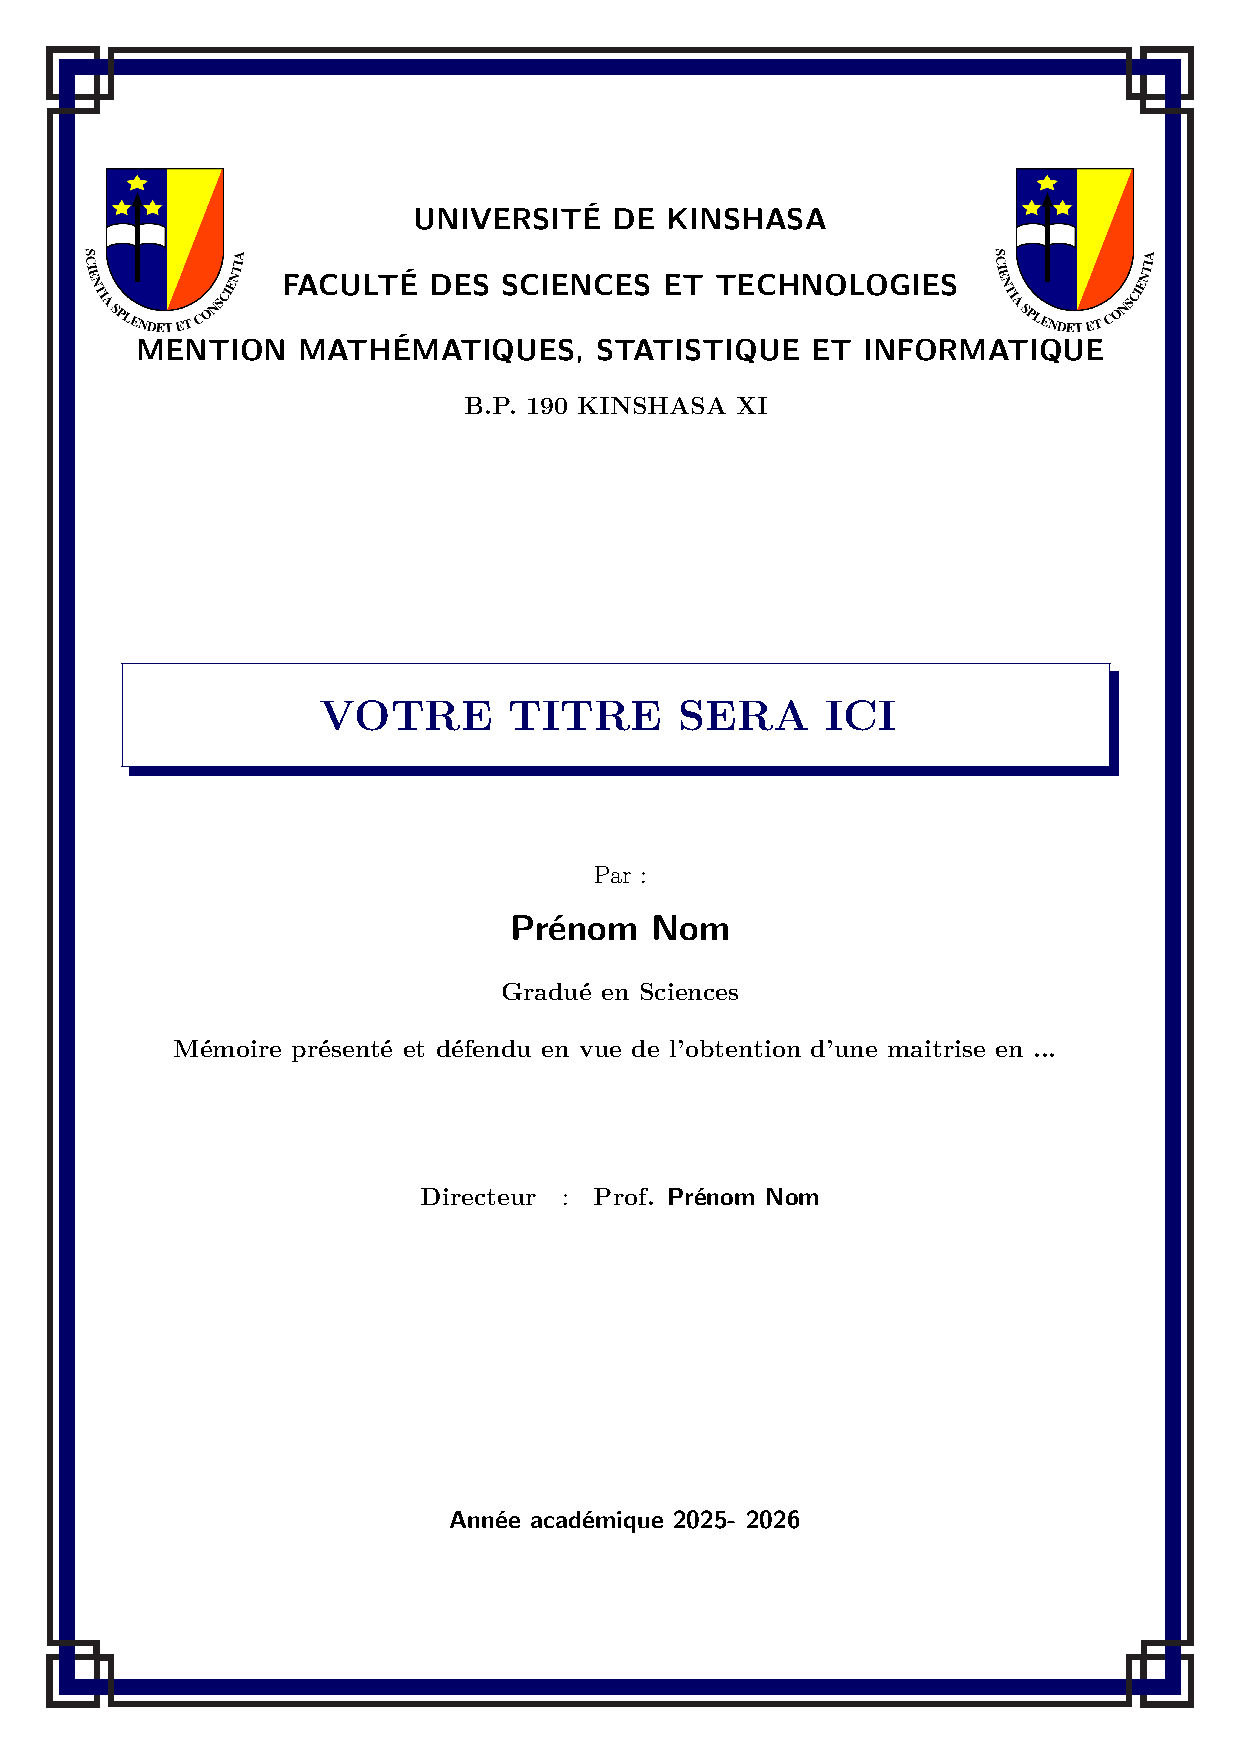
\includepdf[pages=1]{page_de_garde.pdf}
 	\end{titlepage}
 	
 	
 	\chapter*{}
 	
 	\thispagestyle{empty}
 	\pagenumbering{gobble}
 	\vspace{5cm}
 	\begin{flushright}
 		À \bsc{Jean-Pierre} et \bsc{Christine Bien-Aimée}
 	\end{flushright}
 	
 	\frontmatter
 	
 	\chapter*{Remerciements}
 	\addcontentsline{toc}{chapter}{Remerciements}
 	À L'origine ce travail se voulait être le plus sobre possible et dénué de tout sentiment personnel mais la réalisation d'un tel objectif requiert l'usage des connaissances reçues de quelques maîtres grâce notamment aux soutiens de quelques personnes que nous nous devons de mentionner.\\
 	
 	Arrivé au terme de notre second cycle universitaire, nos remerciements à nos parents, \bsc{Jean-Pierre M. Kiakisolako} et \bsc{Christine Bien-Aimée M. Tshamua} pour leur soutien indéfectible et leur patience.\\
 	
 	Nos remerciements à notre Directeur, le Professeur \bsc{Pascal K. Mubenga}, pour sa disponibilité et son dévouement dans la formation de la jeunesse. Nous nous donnons le devoir de transmettre les leçons apprises de lui aux autres à chaque fois que nous en aurons l'occasion.\\
 	
 	Nos remerciements à la \bsc{Fondation Mapon} pour avoir financé nos études. Qu'elle trouve en ces lignes notre gratitude et notre reconnaissance.\\
 	
 	Sacrée étant la famille, nous remercions en ces lignes nos frères et soeurs \bsc{Bienheureuse Kiakisolako}, \bsc{Bien-Faisante Kiakisolako}, \bsc{Bienveillant Kiakisolako}, \bsc{Jêrome Wetu} et \bsc{Sandrine Mansanga}  pour leur soutien. \\
 	Nos remerciements également à \bsc{Joséphine Tshiela} pour son soutien sans lequel nous n'en serons pas arrivé là.\\
 	
 	Pour grandir, il nous a fallu nous tenir sur les épaules des géants. Dans cette démarche nous remercions les géants qui se sont disponibilisés pour nous amener au terme de ce cycle d'études notamment les Professeurs \bsc{Augustin Matata}, \bsc{Alain Musesa}, \bsc{Jean-Paul Tsasa}, \bsc{Samuel Diangitukulu}, \bsc{Jonathan Esole}, \bsc{Efrem Mbaki} et  \bsc{Guillaume Komawila}. \\
 	
 	Enfin, pendant notre parcours nous avons eu la chance de rencontrer ces personnes qui nous ont aimé, motivé, soutenu et encouragé. Les épreuves difficiles traversées ensemble nous rappellent ce que chacun d'entre nous est capable de faire pour les autres et nous rassurent que la famille n'est pas seulement une question de sang.\\
 	De ce fait, nos sincères remerciements à \bsc{Élie Mweze, Jérémie Nlandu, Thierry Tshiebwe, Galilée Kambo, Thérèse Shala, Moïse Saleh, Jeancy Kibata, Pierre Mbungu} et \bsc{Félix Édjobola}.\\ \\
 	
 	\begin{flushright}
 		\bsc{Bien-Aimé J.-P. M. Kiakisolako}
 	\end{flushright}
 	
 	\chapter*{Introduction}
 	\addcontentsline{toc}{chapter}{Introduction}
 	Il existe plusieurs méthodes de résolution des problèmes de Programmation Linéaire Semi-Infinie (PLSI)  dont les méthodes de discrétisation par les parties finies \cite{b2}\cite{b16} et d'autres que l'on retrouve dans la littérature, .\\ 
 	En considérant l'approche utilisée pour trouver la valeur optimale, ces méthodes peuvent être classées en plusieurs catégories parmi lesquelles
 	\begin{enumerate}
 		\item celles qui étudient la convergence des valeurs optimales des sous-problèmes finis vers la valeur optimale du problème de PLSI donné ; 
 		\item celles qui transforment le problème de PLSI donné en un problème de Programmation sans contraintes (en utilisant les multiplicateurs de Lagrange par exemple).  
 	\end{enumerate} 
 	
 	Dans ce travail, l'attention est portée sur l'aspect non pris en compte dans les deux catégories d'approche ci-haut, Nous cherchons la valeur optimale du problème de PLSI en étudiant la convergence des domaines de ses sous-problèmes finis, \ie  en étudiant la convergence des ensembles admissibles des sous-problèmes finis.\\
 	Chaque ensemble  admissible étant convexe et fermé \cite{b16}, suivant quelles topologies ces ensembles  convergent-ils ? À ce niveau nous recourons aux hypertopologies \cite{b8} qui sont définies sur les familles d'ensembles et de ce fait sont mieux indiquées pour étudier la convergence ensembliste.\\
 	Les propriétés des hypertopologies utilisées sont d'abord traitées dans un cadre plus  général puis ramenées au cas d'étude de ce travail \ie sur l'espace $\R^m$.\\
 	
 	Les problèmes de PLSI étant de deux types, le type choisi dans ce travail est le même que celui traité dans \cite{b2}\cite{b22}; Les problèmes de PLSI considérés sont ceux ayant un nombre fini de variables et une infinité de contraintes.\\
 	Toutefois, le nombre de contraintes est infini arbitraire contrairement à \cite{b22} où le nombre de contraintes est supposé infini dénombrable. \\
 	
 	Ce travail est subdivisé en trois chapitres :
 	\begin{enumerate}
 		\item Une introduction aux hypertopologies qu'on peut voir en détails dans \cite{b8}\cite{b7};
 		\item Une introduction à la Programmation Linéaire Semi-Infinie dont les références principales sont \cite{b2}\cite{b8}
 		\item L'application des hypertopologies du chapitre I à la PLSI dont la référence principale est \cite{b21}
 	\end{enumerate}
 	
 
\newpage \tableofcontents


\mainmatter
\chapter{Hypertopologies}
Dans ce chapitre, après une brève introduction à la notion d'hyperespace que le lecteur trouvera en détails dans \cite{b5,b1}, \cite{b6} et \cite{b7},  nous présentons quelques hypertopologies particulières et les propriétés y relatives. Ce champ étant vaste, nous nous limitons aux notions directement liées à ce travail tout en signalant, si nécessaire et dans la mesure du possible, les références pour une étude plus approfondie.\\
Tout au long de ce travail, sauf mention contraire, $X$ représente un ensemble et $\tau$ une topologie sur $X$.
\section{Rappels}
On note $C(X,\R)$, l'espace des fonctions continues sur $X$.
\begin{itemize}[label = $\bullet$]
	\item Soit $(f_n)_{n\in \N}$ une suite dans $C(X,\R)$ et $f \in C(X,\R)$, on dit que $(f_n)$ converge ponctuellement (ou simplement) vers $f$ \ssi $\forall x \in X$, $(f_n (x))_{n \in \N}$ converge vers $f(x)$.\\ 
	On note $C_p (X,\R)$ l'espace des fonctions continues sur $X$ muni de la topologie de la convergence ponctuelle.
	\item 	Un espace topologique $(X,\tau)$ est métrisable s'il existe une métrique $d$ sur $X$ telle que $\tau$ coïncide avec la topologie $\tau_d$ engendrée par $d$.\\ Dans ce cas, $d$ est une métrique compatible avec $\tau$ sur $X$.
	\item Soient $d_1$ et $d_2$ deux métriques sur un ensemble $X \neq \emptyset$. On dit que $d_1$ et $d_2$ sont uniformément équivalentes si $id_X$ est uniformément continue pour $d_1$ et $d_2$ et pour $d_2$ et $d_1$.
	\item Un espace topologique $X$ est accessible ou est un $T_1$-espace si pour tout pair $x,y$ des points de $X$ tels que $x\neq y$, chacun 	admet un voisinage ne contenant pas l'autre. \\
	Dans des tels espaces, tout singleton est fermé \cite{b9}.
	
\end{itemize}
\ \\
Si $(X,\tau)$ est un espace topologique, on note par : 
\begin{enumerate}[label = $\bullet$]
	\item $Fe_{\tau}(X)$, l'ensemble des $\tau$-fermés non vides de X, \ie $$Fe_{\tau}(X) = \lbrace A \subset X :  A \text{ est }  \tau-\text{fermé et non vide} \rbrace$$
	\item $2^X$, l'ensemble des $\tau-$fermés de $X$, \ie $$2^X = \lbrace A \subset X \colon  A \text{ est $\tau$-fermé} \rbrace$$
	\item $FC(X) = \lbrace A \subset X \colon  A \text{ est fermé et convexe} \rbrace$ 
\end{enumerate}
On les appelle les hyperespaces de $(X, \tau)$.\\ \
On peut définir d'autres hyperespaces en considérant, par exemple,  les parties compactes de $X$. Mais nous nous limitons ici aux hyperespaces cités ci-haut.	
\begin{definition}[Hypertopologie]\label{d1}\ 
	Soit $(X,\tau)$ un espace topologique. Une topologie $\psi$ sur $Fe_{\tau} (X)$ est une hypertopologie si l'application 
	$$ \begin{array}{rccl}
		h : & X & \longrightarrow & \lbrace \closure{\lbrace x \rbrace} : x \in X \rbrace  \subset Fe_{\tau} (X) \\
		& x & \longmapsto & \closure{\lbrace x\rbrace}
	\end{array} $$
	est un homéomorphisme de $X$ sur $ \lbrace \closure{\lbrace x \rbrace} : x \in X \rbrace \equiv H$ pour $ \tau$ et $ \psi_{_{H}} \equiv$ topologie induite sur $H$ par $ \psi $.
\end{definition}\ 
Dans ce cas, on dit que $\psi$ est une topologie admissible (compatible avec $\tau$).\\
Une hypertopologie $\psi$ est donc une topologie sur l'hyperespace $Fe_{\tau} (X)$ de $(X,\tau)$ admissible au sens de la définition \ref{d1}.

Cette notion d'uniforme équivalence sera utilisée dans une caractérisation de la topologie proximale.	
\begin{definition}[Hypertopologie]\label{d2}\  
	Si $ (X,\tau) $ est un $T_1$-espace, \ie un espace topologique \textbf{accessible}.
	Une topologie $\psi$ sur $ Fe_{\tau}(X) $ est une hypertopologie si l'application 
	$$ \begin{array}{rccl}
		h : & X & \longrightarrow & \lbrace\lbrace x \rbrace : x \in X \rbrace  \subset Fe_{\tau} (X) \\
		& x & \longmapsto & \lbrace x\rbrace
	\end{array} $$
	est un homéomorphisme de $X$ sur $ \lbrace \lbrace x \rbrace : x \in X \rbrace \equiv H$ pour $ \tau$ et $ \psi_{_{H}} \equiv$ topologie induite sur $H$ par $ \psi $.
\end{definition}\ 
Comme on peut le voir dans \cite{b7}, lorsque l'espace topologique $(X,\tau)$ est accessible, les définitions \ref{d1} et \ref{d2} sont équivalentes.

Pour la commodité dans l'écriture et sans perte de  généralités, nous supposerons toujours l'espace topologique $X$ de départ accessible sachant que dans le cas contraire il suffira de prendre l'adhérence des singletons pour définir l'application $h$ comme en \ref{d1} ci-dessus.\\ 
\begin{definition}[Filtres \cite{b11}]
	Un Filtre sur un ensemble $X$ est une famille $\Fr$ des parties de $X$ vérifiant : 
	\begin{enumerate}[label = $\bullet$]
		\item $\Fr \neq \emptyset$ et $\emptyset \notin \Fr$;
		\item $A\in \Fr$ et $B \in \Fr \Rightarrow A \cap B \in \Fr$;
		\item $A \subset B $ et $A \in \Fr$ $\Rightarrow B \in \Fr$
	\end{enumerate}
\end{definition}
La notion de filtres est souvent accompagnée d'une autre notion que nous présentons ci-dessous.
\begin{definition}[Direction - Ensemble dirigé - Filets ou Suites Généralisées \cite{b11}]\ 
	\begin{enumerate}[label=$\bullet$]
		\item Par une direction sur un ensemble $D$ on entend une relation $\leq$ sur $D$ qui soit réflexive, transitive et telle que pour $a,b \in D$ il existe $c\in D$ avec $a\leq c$ et $b \leq c$.
		\item Par un ensemble dirigé on entend un couple $(D,\leq)$ où $D$ est un ensemble non vide et  $\leq$ une direction sur $D$.
		\item Une suite généralisée ou un filet dans un ensemble $X$ est une fonction définie sur un ensemble dirigé et à valeurs dans $X$.\\
		On écrira "la suite généralisée $(S_t,\ t \in D,\ \leq)$ dans $X$" pour signifier que $(D,\leq)$ est un ensemble dirigé et que $S \colon D \longmapsto X$ avec $S_t = S(t)$ pour tout $t \in  D$.
	\end{enumerate}
\end{definition}
Les notions de Filtres et de Filets sont très liées en ce sens qu'un filtre engendre un filet et qu'un filet engendre un filtre.\\
Clairement, \cite{b11} montre que ces notions sont équivalentes car si $(S_t)_{t\in D}$  est un filet alors le filet engendré par son filtre associé coïncide avec $ (S_t)_{t\in D}$.\\
De même si $\Fr$ est un filtre, le filtre engendré par son filet associé coïncide avec \Fr.\\
Cette équivalence nous permettra donc d'utiliser l'une ou l'autre de ces notions selon le besoin.\\
\begin{definition}[Topologies faibles \cite{b11}]\label{topfaible}
	On se donne des ensembles $E \neq \emptyset$ et $I \neq \emptyset$ ainsi qu'une famille	$\lbrace (Y_t, \tau_t) \colon t \in I \rbrace$ d'espaces topologiques. $\forall t \in I$ soit une application $f_t \colon E \longmapsto Y_t$. Alors il existe une et une seule topologie $\alpha = \sigma(E, \lbrace f_t \colon t \in I \rbrace)$ sur $E$ ayant les deux propriétés suivantes :
	\begin{enumerate}[label = $\bullet$]
		\item $\forall t \in I$, $f_t$ est continue sur $E$ pour $\alpha$ et $\tau_t$;
		\item Si $\delta$ est une topologie sur $E$ telle que chaque $f_t$ est continue sur $E$ pour $\delta$ et $\tau_t$, alors $\alpha$ est plus faible que $\delta$, $\alpha \subset \delta$.
	\end{enumerate}
	$\alpha$ est donc la topologie la plus faible sur $E$ rendant toutes les fonctions $f_t$ continues sur $E$. On l'appelle topologie faible sur $E$ déterminée par les $f_t$ et les $(Y_t, \tau_t)$.
\end{definition}
\section{Quelques hypertopologies}
Nous présentons ici, de manière sommaire, quelques hypertopologies. Leurs constructions détaillées et leurs propriétés peuvent être trouvées dans les livres de référence en  \cite{b5} et \cite{b8} mais aussi dans \cite{b7} pour les trois premières hypertopologies. 

Considérons un espace topologique $(X,\tau)$  avec $X \neq \emptyset$.
\begin{enumerate} 
	\item Si $B$ est un  ouvert de $X$, on définit les ensembles $B^+$, $B^-$ et $\mathcal{B}$ par :\\
	\begin{tabular}{rlcl}
		$\bullet$ &$B^-$ &=&  $\lbrace E \in Fe_\tau (X) : E \cap B \neq \emptyset \rbrace $; \\
		$\bullet$ &$B^+$ &=& $\lbrace E \in Fe_\tau (X) : E \subset B \rbrace$; \\ 
		$\bullet$&$\mathcal{B}$ &= &$\lbrace B^- \colon B \in \tau \rbrace \cup \lbrace (X\setminus K)^+\colon  K\ \text{ compact de } X \rbrace $ 
	\end{tabular}
	%	alors $\mathcal{B}$ est une sous-base d'une topologie sur $Fe_\tau (X)$ qu'on appelle $``$ hypertopologie de Fell$"$ notée $\tau_{\mathcal{F}}$.
	\item Si $V_1,\dots,V_n$ sont des $\tau$-ouverts. On note par :
	\begin{enumerate}[label = $\bullet$]
		\item  $ \langle V_1,V_2,\dots, V_n  \rangle$   $\equiv $~ $\lbrace A  \in  $ $Fe_{\tau}(X)$ : A $ \subset \bigcup_{i=1}^{n} V_i$ ~et ~$ A \cap V_i \neq \emptyset \  \forall i =~ 1,2,\dots,n \rbrace$;
		\item $ \mathcal{A}$ =  $\lbrace \langle V_1,V_2,\dots, V_n \rangle : \ n \in \mathbb{N} \rbrace \subset \wp (Fe_{\tau}(X) )$.
	\end{enumerate}
	%Alors $\mathcal{A}$ est une base d'une topologie sur $Fe_\tau (X)$ qu'on appelle $``$hypertopologie de Vietoris$"$ notée $\tau_v$.
\end{enumerate}  
\begin{definition}[Hit-and-miss hypertopologies] \label{hit}
	Les topologies dont les bases sont formées par les ensembles de type $B^-$ et $B^+$ sont appelées topologies de type \textbf{\textit{hit-and-miss}}.
\end{definition}
\begin{propdf}[Hypertopologie de Vietoris $\tau_v$]\addcontentsline{toc}{subsection}{Hypertopologie de Vietoris $\tau_v$}
	\ 
	\newline
	Soit (X,$ \tau $) un espace topologique accessible avec  $X \neq \emptyset$ et $ \forall n \in \mathbb{N} $; $ V_1 $,$ V_2$,\dots,$ V_n $ des $ \tau $-ouverts de X.\\ 
	Si on note :
	\begin{itemize}
		\item $ \mathcal{A}$ =  $\lbrace \langle V_1,V_2,\dots, V_n \rangle : \ n \in \mathbb{N} \rbrace \subset \wp (Fe_{\tau}(X) )$
		\item $ \tau_v $ = $\tau$($\mathcal{A}$) = $ \left\lbrace \bigcup \mathcal{E} : \mathcal{E} \subset \mathcal{A} \right\rbrace$
	\end{itemize}
	Alors $\tau_v$ est une topologie admissible sur $\Fe$ de base $\mathcal{A}$, \ie une hypertopologie appelée hypertopologie de Vietoris \cite{b7}.
\end{propdf}
\begin{proof}
	\begin{enumerate}
		\item Montrons que $ \bigcup \mathcal{A} = Fe_{\tau}(X)$   .
		\begin{itemize}
			\item Clairement $ \mathcal{A} \subset \wp(Fe_{\tau}(X)) $, on a : $ \bigcup \mathcal{A} \subset Fe_{\tau}(X)$.
			\item $\langle X \rangle$ $ \in \mathcal{A} $ car X $ \in \tau$ or $\langle X \rangle$ = $ Fe_{\tau}(X) $ car : 
			\begin{enumerate}[label=(\roman*)]
				\item $\langle X \rangle$ $ \subset Fe_{\tau}(X) $ par définition;
				\item $ M \in Fe_{\tau}(X)$ $\Rightarrow $ $\emptyset \neq M \subset X $ et $ M \cap X \neq \emptyset $ $\Rightarrow$ M $ \in $  $\langle X \rangle$.
			\end{enumerate}
		\end{itemize} 
		On a donc $ Fe_{\tau}(X) $ =  $\langle X \rangle$ $ \in \mathcal{A} $. \\
		D'où $ Fe_{\tau}(X) \subset \bigcup \mathcal{A} $. Ce qui montre que $ \bigcup \mathcal{A} =  Fe_{\tau}(X)  $
		\item Soient A,B $ \in \mathcal{A} $ et  $ D \in A \cap B $.
		\begin{itemize}
			\item  $ A \in \mathcal{A} \Rightarrow \exists n \in \mathbb{N} \ \exists$ des $ \tau $-ouverts $ V_1,V_2,\dots, V_n  $ tels que $ A = \langle  V_1,V_2, \dots , V_n \rangle  $.
			\item $ B \in \mathcal{A} \Rightarrow \exists m \in \mathbb{N} \ \exists$ des $ \tau $-ouverts $ W_1,W_2,\dots, W_m  $ tels que $B = \langle W_1,W_2, \dots , W_m \rangle $.\\
			$D \in A \cap B \Rightarrow D \in A = \langle V_1,V_2, \dots , V_n \rangle $ et $D \in B = \langle W_1,W_2, \dots , W_m \rangle  $\\ \\ i.e. $\left\lbrace 
			\begin{array}{ll}
				D \subset \cup_{i=1}^{n} V_i \ \mbox{ et } \forall i \in \lbrace 1,\dots,n \rbrace \mbox{, } D \cap V_i \neq \emptyset\\
				D \subset \cup_{i=1}^{m} W_i \mbox{ et } \forall i \in \lbrace 1, \dots ,m \rbrace \mbox{, } D \cap W_i \neq \emptyset
			\end{array}  
			\right.$ \\ \ \\
			Considérons l'ensemble F défini par : \\
			F = $ \langle V_1 \cap \bigcup_{i=1}^{m} W_i, \dots, V_n \cap \bigcup_{i=1}^{m} W_i, W_1 \cap \bigcup_{i=1}^{n} V_i, \dots, W_{m} \cap \bigcup_{i=1}^{n} V_{i}\rangle $, \\ \\  $ F \in \mathcal{A}$ car $\forall i \in \lbrace 1,\dots,n \rbrace $, $V_i \cap \bigcup_{j=1}^m W_j \in \tau$; idem $ \forall j \in \lbrace 1,\dots,m \rbrace $, $W_j \cap \bigcup_{i=1}^n V_i \in \tau$.\\ 
			On montre que $F \subset A \cap B$.\\  \\
			Pour $ G \in F $ on a : \\ 
			$ G \in Fe_{\tau}(X) $ tel que :  \\
			$ G \subset ((V_1 \cap \bigcup_{j=1}^{m} W_j) \cup, \dots, \cup (V_n \cap \bigcup_{j=1}^{m} W_j) \cup (W_1 \cap \bigcup_{i=1}^{n} V_i)\cup , \dots,\cup(W_m ~\cap ~\bigcup_{i=1}^{n} V_i )) $ et $ \forall i \in \lbrace 1, \dots, n \rbrace $, $\forall j \in \lbrace 1, \dots, m \rbrace $ : \\ $ G \cap (V_i \cap \bigcup_{j=1}^{m} W_j) \neq \emptyset  $, $ G \cap (W_j \cap \bigcup_{i=1}^{n} V_i) \neq \emptyset  $\\
			$\Rightarrow G \subset ((V_1 \cup V_2 \cup \dots \cup V_n) \cap \bigcup_{j=1}^{m} W_j) \cup (W_1 \cup W_2 \cup \dots \cup W_m) \cap \bigcup_{i=1}^{n} V_i))$ et $ \forall i\in \lbrace 1, \dots, n \rbrace  $ $ G \cap (V_i \cap \bigcup_{j=1}^{m} W_j) \neq \emptyset  $, $\forall j \in \lbrace 1, \dots, m \rbrace $ $ G \cap (W_j \cap \bigcup_{i=1}^{n} V_i) \neq \emptyset   $ \\
			$\Rightarrow G \subset (\bigcup_{i=1}^{n} V_i \cap \bigcup_{i=1}^{m} W_i) \cup (\bigcup_{i=1}^{m} W_i \cap \bigcup_{i=1}^{n} V_i) $ et $ \ \forall i \in \lbrace 1, \dots, n \rbrace $, \\ $ G \cap (V_i \cap \bigcup_{j=1}^{m} W_j) \neq \emptyset  $, $\forall j \in \lbrace 1, \dots, m \rbrace$ $, G \cap (W_j \cap \bigcup_{i=1}^{n} V_i) \neq \emptyset  $\\ 
			$ \Rightarrow G \subset \bigcup_{i=1}^{n} V_{i} \cap \bigcup_{j=1}^{m} W_{j} $ et $ \forall i \in \lbrace 1, \dots, n \rbrace$ $\exists s \in \lbrace 1, \dots, m \rbrace $ tel que $ G \cap V_{k} \cap W_{s} \neq \emptyset $ et $ \forall j \in ~\lbrace 1, \dots, m \rbrace \ \exists t \in \lbrace 1, \dots, n \rbrace$,  $ G \cap W_{j} \cap V_{t} \neq \emptyset $\\
			$ \Rightarrow G \subset \bigcup_{i=1}^{n} V_i$ et $ G \subset \bigcup_{j=1}^{m} W_{j} $ et $\forall i \in \lbrace 1, \dots, n \rbrace\ G \cap V_k \neq \emptyset$, \\ $\forall j \in \lbrace 1, \dots, m \rbrace$ $ G \cap W_j \neq \emptyset $\\
			$ \Rightarrow G \subset \bigcup_{i=1}^{n} V_{i}$ et $\forall i \in \lbrace 1, \dots, n \rbrace $, $G \cap V_{i} \neq \emptyset$, $ G \subset \bigcup_{j=1}^{m} W_{j} $ et $ \forall j \in \lbrace 1, \dots, m \rbrace $, $ G \cap W_{j} \neq \emptyset $\\
			$ \Rightarrow G \in A$ et $ G \in B $\\
			$ \Rightarrow G \in A \cap B $\\ \\ D'où $ F \subset A \cap B $\\ \\
			Il reste à montrer que $ D \in F $.\\
			$D in A \cap B \Rightarrow$ $\left\lbrace 
			\begin{array}{ll}
				D \subset \bigcup_{i=1}^{n} V_{i} & \mbox{et } \forall i \lbrace 1, \dots, n \rbrace , D \cap V_{i} \neq \emptyset\\
				D \subset \bigcup_{i=1}^{m} W_{i} & \mbox{et } \  \forall j \lbrace 1, \dots, m \rbrace $, $ D \cap W_{j} \neq \emptyset  \\
			\end{array}  
			\right.$\\
			$ \Rightarrow D \subset \bigcup_{i=1}^{n} V_{i} \cap \bigcup_{j=1}^{m} W_{j}   = ((V_1 \cap \bigcup_{j=1}^{m} W_i) \cup (V_2 \cap \bigcup_{j=1}^{m} W_j) \cup, \dots, \cup (V_n \cap \bigcup_{j=1}^{m} W_j) \cup (W_1 \cap \bigcup_{i=1}^{n} V_i)\cup (W_2 \cap \bigcup_{i=1}^{n} V_i) \cup, \dots,\cup(W_m ~\cap ~\bigcup_{i=1}^{n} V_i )) $\\ On a : \\ 
			$ \forall j \in \lbrace 1, \dots, m \rbrace $, $ D \cap (W_{j} \cap \bigcup_{i=1}^{n} V_{i}) = (D \cap W_{j}) \cap (D \cap \bigcup_{i=1}^{n} V_{i}) = (D \cap W_j) \cap D$, $= D \cap W_j \neq \emptyset $\\ $\Rightarrow \forall j \in \lbrace 1, \dots, m \rbrace $, $ D \cap (W_{j} \cap \bigcup_{i=1}^{n} V_{i}) \neq \emptyset $\\ et \\
			$\forall i  \in \lbrace 1, \dots, n \rbrace $, $ D \cap (V_{i} \cap \bigcup_{i=1}^{m} W_{i}) = (D \cap V_{i}) \cap (D \cap \bigcup_{i=1}^{m} W_{i})= (D \cap V_{i}) \cap D $, $= D \cap V_{i} \neq  \emptyset$\\ $\Rightarrow \forall i \in \lbrace 1, \dots, n \rbrace   $, $ D \cap (V_{i} \cap \bigcup_{i=1}^{m} W_{i}) \neq \emptyset $ \\ \\
			Ceci revient à dire que : \\ $D \in  \langle V_1 \cap \bigcup_{i=1}^{m} W_i, \dots, V_n \cap \bigcup_{i=1}^{m} W_i, W_1 \cap \bigcup_{i=1}^{n} V_i, W_2 \cap \bigcup_{i=1}^{n} V_i, \dots, W_{m} \cap \bigcup_{i=1}^{n} V_{i}\rangle$ i.e. $D \in F$.\\
			D'où $  \forall A \in \mathcal{A}\ \forall B \in \mathcal{A} \ \forall D \in A \cap B $, $ \exists F \in \mathcal{A} $ tel que $ D \in F \subset A \cap B $ ce qui montre, par la méthode générale de construction d'une topologie sur un ensemble non vide quelconque \cite{b9}, que $ \tau_{v} $ est une topologie sur $ Fe_{\tau}(X)  $ de base $ \mathcal{A} $.
		\end{itemize}
	\end{enumerate}
	L'application $ h : X \longmapsto $ $ \{\{x\} : x \in X \} $, $ x ~\mapsto $~$ \{x\}$ est un homéomorphisme de $X$ sur $ \lbrace \lbrace x \rbrace : x \in X \rbrace$.
	\begin{enumerate}
		\item L'application h est continue.\\
		Soit $ x \in X $ et H un $\tau_{v}$-voisinage de h($ x $) = $ \lbrace x \rbrace$.\\ $\Rightarrow$ $ \exists$ $ G \in \mathcal{A}$ tel que $ \lbrace x \rbrace \in G \subset H$ (caractérisation des voisinages en termes d'une base).\\
		$ G \in \mathcal{A} \Rightarrow \exists n \in \mathbb{N}$ $\exists$ des $\tau$ ouverts $V_1,V_2, \dots , V_n$ tels que $ G = \langle V_1,V_2, \dots , V_n\rangle$\\ Comme $\lbrace x \rbrace \in G = \langle V_1,V_2, \dots , V_n\rangle $  alors $ \lbrace x \rbrace \subset \bigcup_{i=1}^{n} V_{i}$ et $ \forall k \in \lbrace 1, \dots, n \rbrace $, $\lbrace x \rbrace \cap V_{k} \neq \emptyset$\\
		$\Rightarrow \forall k \in \lbrace 1, \dots, n \rbrace$, $ x \in V_k$ \\ 
		$\Rightarrow x \in \bigcap_{k=1}^{n} V_k \in \tau$ (intersection d'un nombre fini de $\tau$-ouverts).\\
		Posons $ M =  \bigcap_{k=1}^{n} V_k $, M est donc un $\tau$-voisinage de $x$.\\
		Soit $ B \in h[M]$.\\
		$ \Rightarrow \exists x \in M$ tel que $ B = h(x) $\\
		$\Rightarrow B = \lbrace x \rbrace $ avec $ x \in \bigcap_{k=1}^{n} V_k $\\
		$ \Rightarrow B \equiv \lbrace x \rbrace \cap V_k \neq \emptyset \  \forall k \in \lbrace 1, \dots,n \rbrace $ et $ B \subset \bigcup_{i=1}^{n} V_k $\\
		$ \Rightarrow B \in \langle V_1,V_2, \dots , V_n\rangle = G \subset H $\\
		$ \Rightarrow B \in H $\\
		i.e. $ h[M] \subset H $\\
		D'où $ \forall \tau_{v}$-voisinage H de $h(x)$ $\exists \tau$-voisinage M = $\bigcap_{k=1}^{n} V_{k} \ de \ x $ tel que $h[X \cap M ] = h[M] \subset ~H$\\ $ \Rightarrow$ h est continue en $x$ pour $\tau $ et $ \tau_{v}$\\
		D'où h est continue sur X car continue en tout $x \in X$.\\
		\item L'application $ h^{-1}$ : h[X] $ \equiv \lbrace \lbrace x \rbrace : x \in X \rbrace \longmapsto X$, $ \lbrace x \rbrace \mapsto x$ :  est continue sur h[X] pour $ \tau_{v}$ et $ \tau $. \\ Soit $G \in h[X]$ et $A$ un $\tau$-voisinage de $ h^{-1} [ G ].$\\
		$G \in h[X] \Rightarrow \exists x \in X $ tel que $G = \lbrace x \rbrace $ donc $  h^{-1}[G] = x$.\\
		Prenons H = $\langle V \rangle$ avec $ V = int_{\tau} (A)$, $A$  étant un voisinage de $h^{-1}[G] = x$, $ x \in int_{\tau} (A) = V  $ i.e. $G  = \lbrace x \rbrace \subset V$\\
		$ \langle V \rangle  = \lbrace E \in Fe_{\tau}(X) \ : \ E \subset V \rbrace $.\\ Ainsi, $ G = \lbrace x \rbrace \in Fe_{\tau}(X)$ avec $ G \subset V.$ \\
		$\Rightarrow G \in \langle V \rangle  = H \in \mathcal{A}  $\\
		$\Rightarrow H$ est un $\tau_v$-voisinage de $G$.\\ \\
		$y \in h^{-1} [H \cap h[X]] \Rightarrow \exists B \in H \cap h[X] $ tel que $h(y) = B$.\\
		\ \ \ \ \ \ \ \ \ \ \ \ \  $ \Rightarrow B \in H $ et $B \in h[X]$ tel que $B = \lbrace y \rbrace$.\\
		\ \ \ \ \ \ \ \ \ \ \ \ \ $ \Rightarrow  \lbrace y \rbrace \in H $\\
		\ \ \ \ \ \ \ \ \ \ \ \ \ $\Rightarrow \lbrace y \rbrace \subset V = int_{\tau} (A) \subset A $, (par définition de H).\\
		\ \ \ \ \ \ \ \ \ \ \ \ \ $\Rightarrow \lbrace y \rbrace \subset A $\\
		\ \ \ \ \ \ \ \ \ \ \ \ \ $\Rightarrow y \in A $ i.e. $h^{-1} [H \cap h[X]] \subset A $\\
		D'où $ \forall \tau$-voisinage $A$ de $ h^{-1}[G]$ $\exists $ un $\tau_{v}$-voisinage H de $G $ tel que $ h^{-1}[ H \cap h[X]] \subset A$\\
		$\Rightarrow h^{-1}$ est continue en G pour $ \tau_{v} $ et $\tau$ cela $\forall G \in h[X]$.\\
		$\Rightarrow h^{-1}$ est continue sur $h[X]$.\\
		Enfin il est évident que h : $ X \longmapsto \lbrace \lbrace x\rbrace : x \in X \rbrace$ est une bijection d'inverse $ h^{-1}$ définie ci-haut.\\
		$h$ est donc un homéomorphisme sur $X$ et par conséquent $\tau_{v}$ est une hypertopologie.
	\end{enumerate}
\end{proof}
Il est courant de définir les hypertopologies comme étant le supremum de deux topologies une inférieure et l'autre supérieure.\\
Dans ce cas, l'hypertopologie de Vietoris se présente comme étant le supremum de $\tau_v^-$ et $\tau_v^+$, \ie $$\tau_v = \tau_v^- \vee   \tau_v^+$$ où  $\tau_v^-$ est la topologie ayant pour sous-base les $\lbrace B^- \colon B \text{ ouvert de } X \rbrace$ et  $\tau_v^+$ la topologie ayant pour base $\lbrace B^+ \colon B \text{ ouvert de } X \rbrace$. Cette approche est principalement utilisée dans \cite{b8}.

\begin{theorem}\ \label{propr1} 
	Soit (X,$\tau$) un espace topologique. Si $ U\in \tau $ alors $ \lbrace A \in Fe_{\tau}(X) \ : \ A \subset U \rbrace \in \tau_{v}$ \cite{b7}.
\end{theorem}
\begin{proof}
	Soit $U \in \tau $. 
	\begin{itemize}
		\item  On sait, par définition, que $\langle U \rangle \equiv \lbrace  A \in Fe_{\tau}(X) \ : \ A \subset \bigcup_{i=1}^1 U_i $ et $A \cap U_1 \neq \emptyset $ avec $U_1 = U \rbrace$ \\
		$\Rightarrow  \langle U \rangle = \lbrace  A \in Fe_{\tau}(X) \ : \ A \subset U$ et $A \cap U \neq \emptyset \rbrace$\\
		or $A \in Fe_\tau(X)  \Rightarrow A \neq \emptyset $ donc $\emptyset \neq A \subset U \Rightarrow A \cap U \neq \emptyset$\\ d'où $\langle U \rangle = \lbrace  A \in Fe_{\tau}(X) \ : \ A \subset U \rangle$
		\item Comme $U$ est un $\tau$-ouvert,  $\lbrace  A \in Fe_{\tau}(X) \ : \ A \subset U \rangle = \langle U \rangle \in \mathcal{A} \subset \tau_v$.\\ 
		$\Rightarrow \langle  A \in Fe_{\tau}(X) \ : \ A \subset U \rangle \in \tau_v$.
	\end{itemize}
\end{proof}
\begin{theorem} \  \label{propr2}
	Soit $(X,\tau)$ un espace topologique. Si $ V$ est $\tau $-fermé alors $ \lbrace A \in Fe_{\tau}(X) \ : \ A \subset V \rbrace$ est  $\tau_{v}$-fermé \cite{b7}. 
\end{theorem}
\begin{proof}\
	Notons $\mathcal{E} = \lbrace A \in Fe_{\tau}(X) \ : \ A \subset V \rbrace$. Clairement $\mathcal{E} \subset Fe_{\tau}(X)$. \\ Considérons $\mathcal{D} = Fe_{\tau}(X) \setminus \mathcal{E} $.\\
	$\Rightarrow \mathcal{D} = \lbrace A \in Fe_{\tau}(X) \ : \ A \nsubseteq V \rbrace  = \lbrace A \in Fe_{\tau}(X) \ : \ A \subset (X \setminus V)  \rbrace$, V étant $\tau$-fermé, $X \setminus V \in \tau$.  \\
	Montrons que $\mathcal{D} \in \tau_{v}$.\\
	Soit $B \in \mathcal{D}$.\\
	$B \in \mathcal{D} \Rightarrow B \in Fe_{\tau}(X)$ et $ B \subset  X \setminus V $, i.e. $B \cap (X \setminus V) \neq \emptyset $.\\
	Prenons $ \langle X \setminus V \rangle$ = $ \lbrace A \in Fe_{\tau}(X) \ : \ A \subset (X \setminus V) \ et \ A \cap( X \setminus V) \neq \emptyset \rbrace \in \mathcal{A}$,  base de $\tau_{v}$\\
	$\Rightarrow  B \in \langle X \setminus V \rangle \subset \mathcal{D}$ \\
	i.e. $\exists$ $ \langle X \setminus V \rangle  \in \mathcal{A} $ tel que $ B \in \langle X \setminus V  \rangle  \subset \mathcal{D}$\\
	$\Rightarrow \mathcal{D}$ est un $\tau_{v}$-voisinage de B, $\forall B \in \mathcal{D}$\\
	$\Rightarrow \mathcal{D} \in \tau_{v}$\\
	D'où $\mathcal{E} = \mathcal{D}^c =  \lbrace A \in Fe_{\tau}(X) \ : \ A \subset V \rbrace$ est $\tau_{v}$-fermé. \\
\end{proof}


\begin{corollaire}
	Si $(X, \tau)$ est un espace topologique, $ U \in \tau$ et B un $\tau $-fermé de $X$. Par les théorèmes \ref{propr1} et \ref{propr2}, l'hypertopologie de Vietoris contient $\langle U \rangle$ et $\langle X, X \setminus B  \rangle$ dans sa base.
\end{corollaire}


Soit $(X,\tau)$ un espace topologique avec $X \neq \emptyset$. 
Comme ci-haut, prenons 	$$\mathcal{B} = \lbrace B^- \colon B \in \tau \rbrace \cup \lbrace (K^c)^+\colon K\ \text{ compact de } X \rbrace $$ 
Parmi les méthodes de construction d'une topologie,  telles que données dans \cite{b9}, figure celle qui utilise une sous-base. Une sous-base engendre une base qui à son tour engendre une topologie.

Utilisant la notion de sous-base, \cite{b7} montre que  $\mathcal{B}$ est une sous-base d'une topologie admissible sur $Fe_\tau (X)$ appelée $``$hypertopologie de Fell$"$ et notée $\tau_F$.

\begin{propdf}[Hypertopologie de Fell $\tau_F$\label{122}] \addcontentsline{toc}{subsection}{Hypertopologie de Fell $\tau_F$}\ \newline
	Soit $(X,\tau)$ un espace topologique accessible avec $X \neq \emptyset$ et $B$ un  ouvert de $X$. La famille $$\mathcal{B} = \lbrace B^- : B \in \tau \rbrace \cup \lbrace B^+ : B \in \tau\ \text{ et }  B^c\ \text{ est un compact} \rbrace $$ est une sous-base d'une topologie, $\tau_{F}$, sur $Fe_\tau (X)$ appelée $``$hypertopologie de Fell$"$ \cite{b7}.\\
	En notant  $\tau_F^+$ la topologie de base $ \lbrace (K^c)^+\colon K\ \text{ compact de } X \rbrace $, $\tau_F$ se présente sous forme d'une hypertopologie de type \textit{hit-and-miss} $\tau_F = \tau_v^- \vee \tau_F^+$.
\end{propdf}
\begin{proof} \ \newline
	\begin{enumerate}
		\item  Par définition on sait que $\lbrace G^+: G \in \tau\rbrace \subset \mathcal{P}(Fe_{\tau}(X)) $ et $\lbrace G^- : G \in \tau \rbrace  \subset \mathcal{P}(Fe_{\tau}(X)) $.\\ 
		$\Rightarrow \lbrace G^+: G \in \tau\rbrace  \cup  \lbrace G^- : G \in \tau \rbrace \subset \mathcal{P}(Fe_{\tau}(X)) $.\label{1i}\\
		D'où $\mathcal{B} \subset \mathcal{P}(Fe_{\tau}(X)) $.
		
		\item On montre que $\mathcal{D} = \lbrace \bigcap \mathcal{E} : \text{ fini }\equiv \mathcal{E} \subset \mathcal{B} \rbrace$ est une base d'une topologie sur $\Fe$
		\begin{enumerate}
			\item Visiblement $\mathcal{D}= \lbrace \bigcap \mathcal{E} : \text{ fini }\equiv \mathcal{E} \subset \mathcal{B} \rbrace \subset \mathcal{B} \subset \mathcal{P}(\Fe)$ d'après (\ref{1i}) ci-dessus.\\
			Donc $\bigcup \mathcal{D} \subset \Fe$\label{ai}
			\item $X \in \tau$ et $X^+ = \lbrace E \in Fe_\tau (X) : E \subset X \rbrace = \Fe$ de même $X^- = \Fe$ $\Rightarrow X^+ \cap X^- = \Fe$ et $X\setminus X = \emptyset$ est compact.\\
			On a $X^+ \in \mathcal{B}$, $X^- \in \mathcal{B} \Rightarrow X^+ \cap X^- \in \mathcal{D} \Rightarrow X^+ \cap X^- \subset \bigcup \mathcal{D}$.\\
			Or $\Fe = X^+ \cap X^-$, donc $\Fe \subset \bigcup \mathcal{D}$.\label{bi}\\
			(\ref{ai}) et (\ref{bi}) $\Rightarrow \Fe = \bigcup \mathcal{D}$.
		\end{enumerate}
		\item Soient $G,H \in \mathcal{D}$ et $E \in G \cap H$.\\
		$E \in G \Rightarrow \exists i,n \in \mathbb{N}$ $\exists G_1, G_2, \dots,G_i,G_{i+1},G_{i+2}, \dots,G_{i+n} \in \tau $ tels que : \\  $E \in G =  G_1^+ \cap G_2^+ \cap \cdots \cap G_i^+ \cap G_{i+1}^- \cap G_{i+2}^- \cap \cdots \cap G_{i+n}^-$\\
		
		De même, \\ $E \in H \Rightarrow  \exists j,m \in \mathbb{N}$ $\exists H_1, H_2, \dots,H_j,H_{j+1},H_{j+2}, \dots,H_{j+m} \in \tau $ tels que : \\  $E \in H =  H_1^+ \cap H_2^+ \cap \cdots \cap H_j^+ \cap H_{j+1}^- \cap H_{j+2}^- \cap \cdots \cap H_{j+m}^- $\\
		On définit $F$ par : 
		$$F = G_1^+ \cap G_2^+ \cap \cdots \cap G_i^+ \cap  H_1^+ \cap H_2^+ \cap \cdots \cap H_j^+ \cap G_{i+1}^- \cap G_{i+2}^- \cap \cdots \cap G_{i+n}^- \cap H_{j+1}^- \cap H_{j+2}^- \cap \cdots \cap H_{j+m}^-  $$
		et soit $L \in F$.\\
		$\Rightarrow L \in  G_1^+ \cap G_2^+ \cap \cdots \cap G_i^+ \cap  H_1^+ \cap H_2^+ \cap \cdots \cap H_j^+ \cap G_{i+1}^- \cap G_{i+2}^- \cap \cdots \cap G_{i+n}^- \cap H_{j+1}^- \cap H_{j+2}^- \cap \cdots \cap H_{j+m}^- $\\
		$\Rightarrow L \in  G_1^+ \cap G_2^+ \cap \cdots \cap G_i^+ \cap G_{i+1}^- \cap G_{i+2}^- \cap \cdots \cap G_{i+n}^-$ et $L \in H_1^+ \cap H_2^+ \cap \cdots \cap H_j^+ \cap H_{j+1}^- \cap H_{j+2}^- \cap \cdots \cap H_{j+m}^- $\\
		$\Rightarrow L \in G \text{ et } L \in H$\\
		$\Rightarrow L \in G \cap H$\\
		D'où $F \subset G \cap H$.\\ Montrons que $E \in F$.\\
		$E \in G \cap H \Rightarrow E \in  G_1^+ \cap G_2^+ \cap \cdots \cap G_i^+ \cap G_{i+1}^- \cap G_{i+2}^- \cap \cdots \cap G_{i+n}^- \cap  H_1^+ \cap H_2^+ \cap \cdots \cap H_j^+ \cap H_{j+1}^- \cap H_{j+2}^- \cap \cdots \cap H_{j+m}^- $\\
		$\Rightarrow E \in G_1^+ \cap G_2^+ \cap \cdots \cap G_i^+ \cap  H_1^+ \cap H_2^+ \cap \cdots \cap H_j^+ \cap G_{i+1}^- \cap G_{i+2}^- \cap \cdots \cap G_{i+n}^- \cap H_{j+1}^- \cap H_{j+2}^- \cap \cdots \cap H_{j+m}^-  $\\
		$\Rightarrow E \in F$\\
		
		En résumé, $\forall G,H \in \mathcal{D}$ $\forall E \in G \cap H$ $\exists F \in \mathcal{D}$ tel que $E \in F \subset G \cap H$.\\ Ce qui nous permet de conclure, d'après \cite{b9}, que $\mathcal{D}$ est bien une base d'une topologie sur $\Fe$ et donc $\mathcal{B}$ en est une sous-base. Cette topologie sera notée $\tau_F$.
		\item L'application $h : (X,\tau) \longmapsto (\Fe, \tau_F)$, $x \mapsto \lbrace x \rbrace$ est un homéomorphisme.
		\begin{enumerate}
			\item  Soient $x \in X$ et $H$ un $\tau_F$-voisinage de $h(x) = \lbrace x \rbrace$.\\
			$H$ $\tau_F$-voisinage de $\lbrace x \rbrace$ $\Rightarrow $ $\exists \mathcal{D} \in \tau_F$ tel que $\lbrace x \rbrace \in \mathcal{D} \subset H$. \\
			Alors par définition de $\tau_F$, $\exists B \in \tau$ tel que $ \lbrace x \rbrace \in B^+ \cup B^-$\\
			Supposons que $\lbrace x \rbrace \in B^+$ alors $\lbrace x \rbrace \subset B$ $\Rightarrow x \in B \in \tau$.\\ $B$ est donc un $\tau$-voisinage de $x$ et clairement $h(B] \subset H$.\\
			Donc on a $\forall \tau_F$-voisinage $H$ de $h(x)$ $\exists \tau$-voisinage $B$ de $x$ tel que $h[B] \subset H$.\\ \ie  h est continue sur $X$ pour $\tau$ et $\tau_F$.
			\item L'application $h^{-1} : h[X] = \lbrace \lbrace x \rbrace :  x \in X \rbrace \longmapsto X$, $ \lbrace x \rbrace \mapsto h^{-1}({x}) = x $ est continue.\\
			Soit $\lbrace x \rbrace \in h[X]$ et $B$ un $\tau$-voisinage de $h^{-1}(\lbrace x \rbrace) = x$ \\
			Prenons $H = T^+$ avec $\emptyset \neq T = int_{\tau} (B) \in \tau$.\\
			$B$ étant un $\tau$-voisinage de $x$, $x \in int_{\tau} (B) = T \Rightarrow \lbrace x \rbrace \subset T $ or $\lbrace x \rbrace \in \Fe$.\\
			$\Rightarrow \lbrace x \rbrace \in H \in \tau_F$, \ie $H$ est un $\tau_F$-voisinage de $\lbrace x \rbrace$.\\
			Résumé : $\forall \lbrace x \rbrace \in h[X]$ et $\forall \tau$-voisinage $B$ de $h^{-1} (\lbrace x \rbrace)  = x $   $\exists$ un $\tau_F$-voisinage $H = (int_{\tau} (B))^+$  de $\lbrace x \rbrace$ tel que $h^{-1} [H \cap h[X]] \subset B$.\\
			D'où $h^{-1}$ est continue. \\
			On conclut que h est un homéomorphisme et donc $\tau_F$ est une hypertopologie.  
		\end{enumerate}
		
		
	\end{enumerate}
\end{proof}



\begin{definition}[Convergence au sens de Kuratowski]\  \newline
	Soit un filet $(A_n)_{n \in D}$ de parties fermées de $X$.
	\begin{enumerate}[label = $\bullet$]
		\item On définit la limite inférieure, $Li$, et la limite supérieure, $Ls$, de $(A_n)_{n \in D}$ par :
		$$ Li A_n = \lbrace x \in X \colon \exists x_n \in A_n \text{ avec } \lim_{n\mapsto \infty} x_n =x \rbrace$$
		$$Ls A_n = \lbrace x \in X \colon \exists x_{k} \in A_{n_k} \text{ tel que } \lim_{k\mapsto \infty} x_k =x, \ (A_{n_k}) \text{ sous-filet de } (A_n)\rbrace$$ 
		
		\item Si $A$ est un fermé de $X$. On dit qu'un filet $(A_n, n \in D, \leq)$ de fermés de $X$ converge vers $A$ au sens de Kuratowski, qu'on note $K-\lim_{n\mapsto \infty} A_n = A$, si $Ls A_n \subset A \subset Li A_n$, \ie si $Ls A_n = A = Li A_n$ \cite{b8}.
	\end{enumerate}
	
	
	
	
\end{definition}
Le lien existant entre la convergence au sens de Kuratowski et la topologie de Fell est donné dans le théorème et le corollaire suivants :
\begin{theorem}
	Soit $X$ un espace de Hausdorff et $(A_n)_{n\in D}$ une suite dans $2^X$, à supposer que les conditions suivantes sont vérifiées : 
	\begin{enumerate}[label= (\roman*)]
		\item $A \subset Li\ A_n$
		
		\item Pour tout compact $K \subset X$, on a $Ls (K \cap A_n) \subset A$.\\
		Alors $(A_n)_{n \in D}$ $\tau_F$-converge vers $A$.
	\end{enumerate} 
\end{theorem}
\begin{proof}
	La condition $A \subset Li \ A_n$ équivaut à la convergence de $(A_n)$ vers $A$ pour la topologie engendrée par $\lbrace V^- \colon V$ ouvert$\rbrace$. On suppose que (ii) est vérifiée, soit  $K$ un compact inclus dans $X$ et $A_n \cap K \neq \emptyset$. Par la compacité de $K$, $Ls(A_n \cap K)$ est un sous-ensemble non vide de $K$., par la condition (i) , $A \cap K \neq \emptyset$.
	$$A\cap K = \emptyset \Rightarrow A_n \cap K = \emptyset$$
	Ce qui implique que $A= \tau_F-\lim \ A_n$ \cite{b8}.
\end{proof}


\begin{corollaire}
	Soit $X$ un espace de Hausdorff, à supposer que $A \in 2^X$ et que $(A_n)_{n \in I}$ est un suite dans $2^X$. alors :
	\begin{enumerate}
		\item Si $A = K-\lim A_n$, alors $A= \tau_F-\lim A_n$;
		
		\item Si $X$ est localement compact et que $ A =\tau_F-\lim A_n$ alors $A = K-\lim A_n$
	\end{enumerate}
\end{corollaire}
Ainsi, la convergence des suites au sens de Kuratowski décrit la façon dont les suites convergent dans la topologie de Fell \cite{b8,b20}.\\



\begin{propdf}[Métrique de Hausdorff]\label{born1}\  \newline
	Soit $(X,d)$ un espace semi-métrique avec $d$ bornée. $d$ engendre une topologie $\tau_d$ sur $X$ \cite{b9}.\\
	Si $A,B \in Fe_{\tau_d} (X)$ et qu'on définit $H_{d}(A,B)$ par :
	$$H_{d}(A,B) = \max \left\lbrace \sup_{a \in A} d(a,B), \sup_{b \in B} d(b,A) \right\rbrace $$ où $ d(a,H) = \inf \lbrace d(a,x) : x \in H \rbrace$ $\forall H \subset X $ alors $H_d$ est une métrique sur $Fe_{\tau_d} (X)$ \cite{b7}.
\end{propdf}
\begin{proof}\ 
	\newline\ 
	\begin{enumerate}
		
		\item Montrons que $H_d$ est bien définie et positive i.e. $\forall A,B \in Fe_{\tau_{d}}(X), 0 \leq H_d (A,B) \in \mathbb{R}$.
		
		$d$ étant bornée $\exists $ réel $t>0$ tel que $\forall x,y \in X $, $0 \leq d(x,y) \leq t$.\\
		Si $A, B\in Fe_{\tau_{d}}(X)$ :
		\begin{itemize}
			\item $A \neq \emptyset \Rightarrow \exists w \in A$. Alors : \\ 
			$b \in B \in Fe_{\tau_{d}}(X)$ $\Rightarrow 0 \leq d(b,A) = \inf \lbrace d(b,x) : x \in A \rbrace \leq d(b,w) \leq t$.\\
			on a~~ $0 \leq d(b,A) \leq t \  \forall b \in B$. Ce qui signifie que $\emptyset \neq \lbrace d(b,A) : b \in B \rbrace$ est  majoré  par $t$ dans $\mathbb{R}$. Donc $0 \leq \sup \lbrace d(b,A) : b \in B \rbrace \in \mathbb{R}$.
			
			\item $B \neq \emptyset \Rightarrow \exists v \in B $. Alors:\\ 
			$a \in A \in Fe_{\tau_{d}}(X) \Rightarrow 0 \leq d(a,B) = \inf \lbrace d(a,y) : y \in B \rbrace \leq d(a,v) \leq t $.\\  
			On a~~ $0 \leq d(a,v) \leq t \ \forall a \in A$. Ce qui signifie que  $\emptyset \neq \lbrace d(a,v) : a \in A \rbrace$ est majoré par $t$ dans  $\mathbb{R} $. Donc $0 \leq \sup \lbrace d(a,v) : a \in A \rbrace \in \mathbb{R}$.\\
			
			Ainsi, on a :
			$$0 \leq \max \left\lbrace \sup_{a \in A} d(a,B), \sup_{b \in B} (b,A) \right\rbrace \in \mathbb{R}$$
			
			D'où $ H_d \ : \ Fe_{\tau_d}(X) \times Fe_{\tau_{d}}(X) \longrightarrow \mathbb{R} $ avec $0 \leq H_{d}(A,B)$
		\end{itemize}
		
		\item Montrons que $H_d$ vérifie la stricte positivité i.e. $H_d (B,B) = 0$, $\forall B \in~ Fe_{\tau_d}(X) $.
		
		Soit $b \in B$. $b \in B \Rightarrow d(b,B) = 0 $ $\Rightarrow \lbrace d(b,B) : b \in B \rbrace = \lbrace 0 \rbrace$\\
		On a~~ $\sup \lbrace d(b,B) : b \in B \rbrace = \sup \lbrace 0 \rbrace = 0 $\\ 
		Donc $H_d (B,B) = \max \left\lbrace \sup_{b \in B} d(b,B), \sup_{b \in B} d(b,B) \right\rbrace = \max \lbrace 0, 0 \rbrace = 0$\\
		D'où $H_d (B,B) = 0 \ \forall B \in Fe_{\tau_{d}}(X) $.
		\item Montrons que $H_d$ est symétrique i.e. $H_d (A,B) = H_d (B,A) \ \forall A,B \in Fe_{\tau_{d}}(X).$\\
		
		
		$H_d (A,B) =  \max \lbrace \sup_{a \in A} d(a,B), \sup_{b \in B} d(b,A) \rbrace = \max \lbrace \sup_{b \in B} d(b,A), \sup_{a \in A} d(a,B)\rbrace $ $= ~H_{d} (B,A)  $
		
		\item  Enfin montrons que $H_d$ vérifie l'inégalité triangulaire i.e. $ \forall A,B,C \in Fe_{\tau_d}(X)$ \\ $  H_d (A,C) \leq H_d (A,B) + H_d (B,C) \ $
		
		\begin{enumerate}
			\item Si $a \in A,\ b \in B,\ c \in C$, avec d une semi-métrique, on a : \\ $d(a,c) \leq d(a,b) + d(b,c)$\\
			$d(a,b) \leq \max \left\lbrace \sup_{a \in A} d(a,B), \sup_{b \in B} d(b,A) \right\rbrace = H_d (A,B)$ 
			et \\  $ d(b,c) \leq \max \left\lbrace \sup_{b \in B} d(b,C), \sup_{c \in C} d(c,B) \right\rbrace = H_d (B,C)$\\
			$\Rightarrow d(a,b) + d(b,c) \leq  H_d (A,B) + H_d (B,C)$\\
			$\Rightarrow d(a,c) \leq d(a,b) + d(b,c) \leq H_{d} (A,B) + H_{d} (B,C)$\\
			$\Rightarrow d(a,c) \leq H_{d} (A,B) + H_{d} (B,C)$ $\forall a \in A$ $\forall c \in C$\label{idem1}
			\item En raisonnant de la même façon, on a aussi $d(c,a) \leq H_{d} (A,B) + ~H_{d} (B,C)$ \label{idem2}\\
			De 4(a) et 4(b), on obtient : \\
			$H_d (A,C) = \max \left\lbrace \sup_{a \in A} d(a,C), \sup_{c \in C} d(c,A) \right\rbrace \leq H_{d} (A,B) + H_{d} (B,C) $\\ \\
			D'où $H_d (A,C) \leq H_d (A,B) + H_d (B,C) $
		\end{enumerate}
		\item $H_d (A,B) = 0 \Rightarrow A = B$\\ Soient $A,B \in Fe_{ \tau_d} (X)$.
		\begin{enumerate}
			\item $0 \leq \sup_{a \in A} d(a,B) \leq \max \left\lbrace \sup_{a \in A} d(a,B), \sup_{b \in B} d(b,A)\right\rbrace = H_{d} (A,B) = 0 $\\ $\Rightarrow \sup_{a \in A} d(a,B) = ~0 $\\
			
			Soit $ x \in A$, \\
			$d(x,B) \leq \sup_{a \in A} d(a,b) = 0 \Rightarrow d(x,B) = 0$ \\ $\Rightarrow x \in \overline{B} = B  $\\ $\Rightarrow x \in B$, i.e. $A \subset B$
			\item Avec un raisonnement analogue, on trouve que $B \subset A$.\\
			D'où $A = B$
		\end{enumerate}
	\end{enumerate}
\end{proof}
\begin{corollaire}
	Si d est une semi-métrique pas nécessairement bornée sur $X \neq \emptyset.$ La fonction $ \varphi (x,y) = ~\frac{d(x,y)}{1 + d(x,y)}$ est une semi-métrique bornée sur $X$ qui engendre la même topologie que d, i.e. $\tau_{d} = \tau_{\varphi}$.
\end{corollaire}
\begin{proof} \ 
	\newline
	Pour tout $ x,y \in X,\ 0 \leq \varphi(x,y)= \frac{d(x,y)}{1 + d(x,y)} \leq 1 $.\\ \\
\end{proof} 
Dans  ce cas, la métrique $H_{d}$ construite à partir de la semi-métrique bornée $\varphi$ comme dans \ref{born1}.
\begin{definition}
	La métrique $H_d$ ainsi définie sur $Fe_{\tau_d} (X)$ est appelée métrique de Hausdorff.	
\end{definition}
Si $\epsilon$ est un réel strictement positif et $A \in Fe_\tau (X)$, les boules ouvertes et fermées sont définies par ; 
\begin{itemize}
	\item $B(A,\epsilon,H_d,Fe_\tau (X)) = \lbrace B \in  Fe_\tau (X)  : H_d(A,B) < \epsilon \rbrace $, 
	\item $\overline{B} (A,\epsilon,H_d,Fe_\tau (X)) =  \lbrace B \in  Fe_\tau (X)  : H_d(A,B)  \leq\epsilon \rbrace $.
	\item $N_d (A, \epsilon,d, X) = \lbrace x \in X$ : $d(x, A) < \epsilon \rbrace$
\end{itemize}  L'espace métrisable $(X,\tau_d)$ est évidemment accessible, on a $\forall x \in X,\ \lbrace x \rbrace$ est fermé.
\begin{propdf}\addcontentsline{toc}{subsection}{Hypertopologie de Hausdorff $\tau_{H_d}$}\  \
	\newline \
	La topologie $\tau_{_{H_{d}}}$ engendrée par la métrique de Hausdorff $H_d$ sur $Fe_{\tau_d}$ est une hypertopologie appelée hypertopologie de Hausdorff.
\end{propdf}
\begin{proof} \ 
	\newline
	Soit $h : (X, d) \longmapsto (Fe_{\tau_{d}}(X), H_{d})$, $x \mapsto \lbrace x \rbrace$.\\
	Si $x,y \in X$,  $H_d (h(x), h(y)) = H_d ( \lbrace x \rbrace, \lbrace y \rbrace) = \max \left\lbrace \sup_{a \in A} d(a,\lbrace y \rbrace), \sup_{b \in B} d(b,  \lbrace x \rbrace) \right\rbrace $ \\ $ = \max \lbrace \sup d(x,y),\sup d(x,y) \rbrace = \max \lbrace d(x,y), d(x,y) \rbrace = d(x,y) $\\
	$\Rightarrow H_{d} (h(x), h(y)) = d(x,y)$ $\forall x,y \in ~X$, i.e. h est une isométrie sur $X$ pour d et $H_d $\\
	$\Rightarrow$ h est continu sur  $ X $ pour $ \tau_d$ et $ \tau_{_{H_d}}$ \cite{b9}.\\
	De même $ h^{-1} : h[X] = \lbrace \lbrace x \rbrace : x \in X \rbrace \longmapsto X  $ est une isométrie sur $h[X]$ pour $\tau_{_ {H_d}}$ et $\tau_d$\\
	$\Rightarrow h$ est un homéomorphisme de $ X $ sur $h[X]$\\
	D'où $\tau_{_ {H_{d}}}$ est une hypertopologie.  
	
\end{proof}
Cette hypertopologie diffère des premières car elle est engendrée par une métrique. La construction d'une topologie à partir d'une semi-métrique est faite dans \cite{b9} (sa base étant la famille des boules ouvertes relativement à cette semi-métrique).\\
%%%%%%%%%%%%%%%%%%%%%%%%%%%%%%%%%%%%%%%%%
%
%%%%%%%%%%%%%%%%%%%%%%%%%%%%%%%%%%%%%%%%%
%
%%%%%%%%%%%%%%%%%%%%%%%%%%%%%%%%%%%%%%%%%
%																	
%%%%%%%%%%%%%%%%%%%%%%%%%%%%%%%%%%%%%%%%%

\begin{definition}[Inclusion forte - éloignement]\
	Soit $(X,d)$ un espace métrique. 
	\begin{enumerate}[label=$\bullet$]
		\item Étant donné un réel $\epsilon >0$, on définit l'ensemble $S_\epsilon [A]$ par $$S_\epsilon [A] = \lbrace x \in X \colon d(x,A) < \epsilon \rbrace$$
		\item 	Soit $E \subset X$ et un ensemble $\emptyset \neq A \subset X$. On dit que $A$ est fortement inclus dans $E$ s'il existe un réel $\epsilon >0$ tel que $S_\epsilon [A] \subset E$.
		\item Pour tout $B \subset X$, on notera par $B^{++}$ l'ensemble 
		$$B^{++} = \lbrace A \in \Fe \colon \exists \epsilon > 0 \text{ tel que } S_\epsilon [A] \subset B \rbrace$$
		\item 	Étant donné deux ensembles $A$ et $E$, on dit que $A$ est éloigné de $E$  si $A \subset  (E^c)^{++}$.
	\end{enumerate}
\end{definition}

\begin{propdf}\addcontentsline{toc}{subsection}{\textit{Proximal Ball Topology} $\tau_{B_d}$}
	Soit $(X,d)$ un espace métrique. La proximal ball topology $\tau_{B_d}$ sur $\Fe$ est la topologie sur $\Fe$ ayant pour sous-base les ensembles de la forme $V^-$ et $(B^c)^{++}$ où $V$ est un ouvert de $X$ et $B$ une boule fermée de $X$.
\end{propdf}
Il s'agit d'une topologie de type \textit{hit-and-miss} comme on peut le remarquer.\\

Soit $(X,d)$ un espace métrique. En analyse classique, on définit la distance, $d(x,A)$,  d'un point $x \in X$ à un ensemble non vide $A$ comme une fonction de $x$ en maintenant l'argument $A$ fixe. Cependant, on peut également définir $d(x,\cdot)$ en faisant  varier l'argument $A$ dans $\Fe$  et en maintenant $x$ fixe. \\
Pour tout $x \in X$, nous obtenons alors les fonctions $d(x,\cdot) \colon \Fe \longmapsto \R$.

On définit la topologie de Wijsman comme étant la topologie faible déterminée par les fonctions  $\lbrace d(x,\cdot )\colon x \in ~X \rbrace$.
\begin{definition}[Hypertopologie de Wijsman $\tau_{W_d}$]\label{def118}\label{125}\addcontentsline{toc}{subsection}{Hypertopologie de Wijsman $\tau_{W_d}$}
	Soit $(X,d)$ un espace métrique. La topologie de Wijsman, $\tau_{W_d}$, est la topologie faible déterminée par la famille $\lbrace   d(x,\cdot )\colon x \in X \rbrace$ \cite{b8}.
\end{definition}\ 
Comme le montre \cite{b8}, la topologie $\tau_{W_d}$ sur $\Fe$ est admissible, on l'appelle l'hypertopologie de Wijsman.\\
Dans \cite{b8} et \cite{b13} une autre formulation de l'hypertopologie de Wijsman est donnée sous forme d'une hypertopologie de type \textit{hit-and-miss}.
\begin{definition}\label{wijs}
	Dans les conditions de la définition \ref{def118} précédente, l'hypertopologie de Wijsman est la topologie sur $\Fe$ ayant pour sous-base les ensembles de la forme $V^-$ où $V$ est un ouvert et les ensembles de la forme $(B^c)^{++}$ où $B \in \Fe$ \ie $$\tau_{W_d} = \tau_V^-  \vee \tau_W^+$$
\end{definition}
\begin{definition}[Convergence au sens de Wijsman]
	Soit $(X,d)$ un espace métrique. Un filet $(A_t)$ dans $\Fe$ converge vers $A \in Fe_{\tau_d}(X)$ au sens de Wijsman, qu'on écrit $A=W_d-\lim A_t$, si pour tout $x \in X$, on ~a $$d(x,A) = \lim_{t\mapsto +\infty} d(x,A_t)$$ 
\end{definition}
Dans \cite{b12} l'hypertopologie de Wijsman  est définie comme étant topologie que $Fe_{\tau_d}$ hérite de $C_p(X,\R)$ par l'identification $A \mapsto d(\cdot, A)$.
\begin{definition}[La Topologie Proximale $\tau_{\delta_d}$]\addcontentsline{toc}{subsection}{La Topologie Proximale $\tau_{\delta_d}$}
	Soit $(X,d)$ un espace métrique. La topologie proximale $\tau_{\delta_d}$ sur $\Fe$ est la topologie sur $\Fe$ ayant pour sous-base les ensembles de la forme $V^-$ où $V$ est un ouvert de $X$ et les ensembles de la forme $W^{++}$ où $W$ est un ouvert de $X$.
\end{definition}
La topologie proximale peut être définie comme la topologie faible engendrée par les métriques uniformément équivalentes à $d$ comme le montre le théorème suivant : 

\begin{theorem}\label{th122}
	Soit $(X,d)$ un espace métrique et $\mathcal{D}_d$ l'ensemble des métriques uniformément équivalentes à $d$. La topologie faible déterminée par la famille des distances $\lbrace \rho(x,\cdot) \colon x \in X, \ \rho \in \mathcal{D}_d \rbrace$ coïncide avec la topologie proximale \cite{b8}.\\
	Un filet $(A_t)$ dans $\Fe$ $\tau_{\delta_d}$-converge vers $A \in \Fe$ \ssi $\forall x \in X$, $\forall d \in \mathcal{D}_d$, $$d(x,A) = \lim_t d(x,A_t)$$
\end{theorem}
\begin{proof}
	Notons par $\sigma$ la topologie faible engendrée par  la famille $\lbrace \rho(x,\cdot) \colon x \i  X,\ \rho \in D_d\rbrace$.\\
	Pour tout $\rho \in D_d$, on a $\tau_{\delta_d} = \tau_{\delta_\rho} \supset \tau_{w_\rho}$ de sorte que $\tau_{\delta_d} \supset \bigwedge \lbrace \tau_{w_\rho} \colon \rho \in D_d \rbrace = \sigma$.\\
	Pour l'inclusion réciproque $\tau_{\sigma_d} \subset \sigma$, on montre que $W^{++} \in \sigma$ pour tout ouvert $W$. Donnons-nous un $A \in W^{++}$ et $\epsilon <\frac{1}{2}$ tel que $S_{2\epsilon} [A] \subset W$.\\
	Il existe $\rho  \in D_d$ tel que 
	\begin{equation}\label{D_d}
		A \in \lbrace B \in \Fe \colon \rho(x_0,A)-\epsilon < \rho(x_0,B)\rbrace \subset S_\epsilon [A]^+ \subset S_{2\epsilon}[A]^++ \subset W^{++}
	\end{equation}
	$\lbrace B \in \Fe \colon \rho(x_0,A) -\epsilon < \rho(x_0,B)\rbrace \in \tau_{w_\rho} \subset \sigma$ cela montrerait que $W^{++} \in \sigma$.\\
	Considérons $\varphi \colon X \mapsto \R$ définie par 
	$$\varphi(x) = \left \lbrace \begin{array}{ccl}
		d(x,A) & \text{ si } & x \in S_\epsilon [A]\\ \\
		\epsilon &  & \text{autrement}
	\end{array}\right.$$
	$\varphi$ étant lipschitzienne de constante $1$, il est uniformément continu, la métrique  $\rho$ définie par $$\rho (x,\omega) = \min \left\lbrace \frac{1}{2}, d(x,y) + \cfrac{1}{\epsilon} \lvert \varphi(x) - \varphi(\omega)\rvert \right\rbrace$$ est uniformément équivalente à $d$.\\
	Si l'inclusion en \ref{D_d} est fausse alors on peut trouver $B  \in \Fe$ tel que $\rho (x_0,A)-\epsilon < \rho(x_0,B) $ et un point $b \in B \cap S_\epsilon [A]^c$. si $x_0 \in W^c \subset S_\epsilon [A]^c$; alors $x_0$ et $b$ sont dans $S_\epsilon [A]^c $ et $\epsilon <\frac{1}{2}$. On a  
	
	
	$$1 \leq \rho(x_0,A) < \rho (x_0,B) + \epsilon \leq \rho (x_0,b) +  \epsilon \leq \frac{1}{2} + \epsilon < 1$$
	Ce qui est absurde, l'inclusion (\ref{D_d}) est donc vraie et $\tau_{\delta_d} \subset \sigma$ .
\end{proof}\ \\
Les problèmes d'optimisation convexes sont très étudiés dans la pratique. Le besoin d'une hypertopologie particulière sur la famille des ensembles fermés et convexes s'est fait ressentir dès l'aube de l'application des hypertopologies dans l'optimisation.

L'hypertopologie de Mosco est une hypertopologie de type \emph{hit-and-miss}, telle que signalée en \ref{hit}, qui prend en compte cet aspect particulier de convexité, elle est définie sur l'ensemble $FC(X)$ des parties fermées et convexes de $X$.\\
Comme toute hypertopologie, l'hypertopologie de Mosco donne lieu à la convergence dite \textbf{convergence à la Mosco}.
\begin{definition}[Hypertopologie de Mosco $\tau_M$]\addcontentsline{toc}{subsection}{Hypertopologie  de Mosco $\tau_M$}
	Soit $X$ un espace normé. On appelle hypertopologie de Mosco, notée $\tau_M$, la topologie sur  $FC(X)$ ayant pour sous-base les ensembles de la forme $\lbrace V^- \colon V \text{ouvert pour la norme } \rbrace$ et $\lbrace (K^c)^+ \colon K \text{ faiblement compact} \rbrace$.\\
	Elle se présente également comme le supremum des topologies de Fell $\tau_F^s$ et $\tau_F^\omega$ définies à partir des topologies fortes et faibles respectivement : $$ \tau_M = \tau_F^s \vee \tau_F^w$$
\end{definition} 
\begin{lemme}
	Soit $X$ un espace normé. L'hypertopologie de Mosco est une topologie de type \emph{hit-and-miss}. Elle possède la même partie inférieure que l'hypertopologie de Vietoris \cite{b23}.
	$$\tau_M = \tau_V^- \vee \tau_M^+$$
\end{lemme}


%On rappelle que $C(X,\R)$ est lespace des fonctions continues sur $X$.
%\subsection{La Topologie de Attouch-Wets}
%{Soit $(X,d)$ un espace métrique. La topologie de Attouch-Wets, $\tau_{AW_d}$, sur $\Fe$ est la topologie qu'hérite $\Fe$ de $C(X,R)$ muni de la topologie $\tau_{cu}$ de la convergence uniforme, par l'identification $A \mapsto d(\cdot, A)$, $\forall A$ fermé de $X$ \cite{b8}.
	
	\section{Comparaison des hypertopologies}
	\begin{theorem}[$\tau_v$ et $\tau_{H_d}$]\label{31}
		Soit (X,d) un espace métrique compact et $\tau$ la topologie engendrée par d. Alors l'espace $(Fe_{\tau} (X)$, $\tau_v)$ est métrisable et $\tau_{v}$ = $\tau_{H_d}$ \cite{b7}.
	\end{theorem}
	\begin{proof}
		\begin{enumerate}
			\item $\tau_{v} \subset  \tau_{H_d}$\\
			Il suffit de montrer que $\langle U \rangle \in \tau_{H_d}$ et $\langle X, U \rangle \in  \tau_{H_d}$  $\forall U \in \tau$ (à cause du lemme \ref{31} précédent .
			\begin{itemize}
				\item Montrons que $\langle U \rangle \in \tau_{H_d}$.\\
				Si $U = X$ alors $\langle U \rangle  = \lbrace A \in Fe_{\tau}(X) : A \subset X \rbrace = Fe_\tau (X)  \in \tau_{H_d}$.\\ 
				Prenons le cas où $U \neq X$ et soit $A \in \langle U \rangle$, \\ Signalons que $A \equiv$ fermé inclus dans le compact $X$ est compact \cite{b9}.\\
				$\epsilon = d(A, X \setminus U) = \inf \lbrace d(a,x) : a \in A$ et $ x \in (X \setminus U) \rbrace $ est un réel $> 0$. \\ Ce réel existe car $A$ est un compact inclus dans l'ouvert $U$ , $A \neq \emptyset$ et $X \setminus U \neq \emptyset$.\\
				Si $B \in B(A,\epsilon, H_d, Fe_\tau (X))$ alors $H_d (A,B) < \epsilon$  et $B \subset N_d (A, \epsilon, d, X)$ ce qui, d'après le choix de $\epsilon$,  montre que $B \subset U$  i.e. $B \in \langle U \rangle$.\\ En résumé, $\forall A \in \langle U \rangle$ $ \exists$ réel $\epsilon > 0$ tel que $B(A, \epsilon, H_d, Fe_\tau (X)) \subset  \langle U \rangle $.\\
				D'où $\langle U \rangle  \in \tau_{H_d}$.
				
				\item Montrons que $\langle X, U \rangle \in  \tau_{H_d} $\\
				Considérons $A \in \langle X, U \rangle$.
				\\  Alors $A \cap U \neq \emptyset$, soit donc $\omega  \in  A \cap U$.\\ $\omega \in U$ et $U \in \tau$ $\Rightarrow \exists$ réel $\delta > 0 $  tel que  $N(\lbrace p \rbrace, \delta, d, X) \subset U$.\\
				Soit $B \in B(A, \delta, H_d, Fe_\tau (X)).$ Alors $H_d (A, B)  < \delta \Rightarrow A \subset N(B, \delta, d, X) $, comme $p \in A$, il existe $b \in B$ tel que $d(p,b) < \delta$ ce qui, d'après notre choix de $\delta$, signifie que $b \in U$. Donc $B \cap U  \neq \emptyset$ ce qui implique, par définition que $B \in \langle X, U \rangle  $ et donc$B(A, \delta, H_d, Fe_\tau (X)) \in \langle X, U \rangle $ \\ D'où $\forall A \in \langle X, U \rangle$ $\exists$ réel $\delta > 0$ tel que $B(A, \delta, H_d, Fe_\tau (X)) \in \langle X, U \rangle$; i.e  $\langle X, U \rangle \in \tau_{H_d}$
			\end{itemize}
			
			\item $\tau_{H_d} \subset \tau_v$\\ 
			Il suffit de montrer que toute boule ouverte suivant $H_d$ est un $\tau_v$-ouvert, i.e. $\forall A \in Fe_\tau (X) $ $ \forall $ réel $t > 0$, il existe un nombre fini de $\tau$-ouverts $U_1, U_2,\cdots, U_n$ tel que : $$A \in \langle  U_1,\cdots, U_n \rangle \subset B(A, t, H_d, Fe_\tau (X))$$
			Soit $A \in  Fe_\tau (X)$ et $t$ un réel $> 0$ alors comme $A$ est compact non vide, il existe un nombre fini de $\tau$-ouvert $U_1, U_2,\cdots, U_n$ tel que : 
			\begin{enumerate}
				\item $A \subset \bigcup_{i=1}^{n} U_i$;\label{com1}
				\item $A \cap U_i \neq \emptyset$ $ \forall i \in \lbrace 1, \cdots, n \rbrace$;\label{com2}
				\item diam $(U_i) <  t $  $\forall i \in \lbrace 1, \cdots, n \rbrace$ \label{com3}
			\end{enumerate}
			(\ref{com1})  et (\ref{com2}) montrent, par définition, que $A \in \langle  U_1,\cdots, U_n \rangle$.
			Si $M \in \langle  U_1,\cdots, U_n \rangle$ alors $M \subset   \bigcup_{i=1}^{n} U_i$, il suit d'après  (\ref{com2}) et (\ref{com3}) que  : $$M \subset N(A, t, d, X)$$
			Aussi, comme $M \cap U_i \neq \empty  \forall i \in \lbrace 1, \cdots, n \rbrace$, (\ref{com1}) et (\ref{com3}) impliquent que ; $$A \subset N(M, t, d, X) $$
			ce qui implique  que $H_d (A,M) < t$, \\ i.e.  $M \in B(A, t, H_d, Fe_\tau (X))$.\\ $\Rightarrow$ $ \langle  U_1,\cdots, U_n \rangle \subset  B(A, t, H_d, Fe_\tau (X))$.\\
			Résumé : $\forall A \in Fe_\tau (X) $ $\forall $ réel $t > 0$ il existe un nombre fini des $\tau$-ouverts $U_1 ,\cdots, U_n$ tel que $A \in \langle  U_1,\cdots, U_n \rangle \subset B(A, t, H_d, Fe_\tau (X))$. En d'autres termes, toute  boule ouverte est un $\tau_v$-ouvert d'où $\tau_{H_d} \subset \tau_v$.
		\end{enumerate}
		D'où l'égalité.
	\end{proof}
	\begin{corollaire}
		Si $(X, \tau)$ est un espace topologique compact et  métrisable alors l'espace $(Fe_\tau (X), \tau_v)$ est métrisable. Si on note $d$ la métrique qui engendre $\tau$ alors $\tau_v = \tau_{H_d}$ \cite{b7}.
	\end{corollaire}
	L'hypertopologie de Vietoris sur les fermés d'un espace métrisable peut être présentée comme une topologie faible, spécialement comme une topologie engendrée par une famille des fonctions distances obtenues en faisant varier les métriques et les points \cite{b14}.
	
	\begin{theorem}\label{th125}
		Soit $(X,\tau)$ un espace métrisable et $\mathcal{D}$ l'ensemble  des métriques compatibles avec $\tau$ sur $X$. Alors la topologie de Vietoris $\tau_v$ sur $\Fe$ est la topologie faible déterminée par la famille des fonctions distances \cite{b8} $$\lbrace d(x,\cdot) \colon x \in X,\ d \in \mathcal{D} \rbrace$$ 
	\end{theorem}
	
	\begin{proof}
		On note par $\sigma$ la topologie faible engendrée par la famille $\mathcal{D}$.\\
		Pour montrer que $\sigma \subset \tau_v$, soit $d \in \mathcal{D}$ et fixons-nous $x \in X$. Pour tout réel $\alpha >0$, $\lbrace B \in \Fe \colon d(x,B) w \alpha \rbrace = S_\alpha [x]$ est un élément de $\tau_v$. \\
		D'une autre part, si $A \in \lbrace \in \Fe \colon d(x,B)> \alpha\rbrace$ alors pour un $\beta > \alpha$, on a $A \cap \overline{S}_\beta [x] = \emptyset$.\\
		Alors $$A \in (\overline{S}_\beta [x])^c)^+ \subset \lbrace B \in \Fe \colon d(x,B) >0 \rbrace$$
		Cela prouve que  chaque membre d'une sous-base de $\tau_{W_d}$ appartient à $\tau_v$. D'où $\sigma \subset \tau_v$ .
	\end{proof}
	
	
	\begin{corollaire}[$\tau_v$ et  $\tau_{W_d}$]\label{co134}
		Si $(X,\tau)$ est un espace métrisable, l'hypertopologie de Vietoris est le supremum de l'ensemble des hypertopologies de Wijsman déterminées par des métriques compatibles avec $\tau$ sur $X$. Un filet $(A_\lambda, \lambda \in D, \leq)$ dans $\Fe$ $\tau_v$-converge vers $A \in \Fe$ \ssi $\forall x \in X$ $\forall d \in \mathcal{D}$, on a $$d(x,A) = \lim_\lambda d(x,A_\lambda)$$
		Par conséquent, pour toute métrique $d \in \mathcal{D}$, $\tau_{W_d} \subset \tau_v$.
	\end{corollaire}\ 
	
	En tant que topologies faibles définies en \ref{th122} et \ref{th125}, la topologie de Vietoris est plus fine que la topologie proximale car $\tau_v$ est définie par une classe des fonctions plus large.
	\begin{theorem}[$\tau_v$ et $\tau_{\delta_d}$]
		Soit $(X,d)$ un espace métrique. Alors $\tau_v = \tau_{\delta_d}$ sur $\Fe$ \ssi pour tout $A, B \in \Fe$ disjoints, $A$ et $B$ sont éloignés \cite{b8}.  
	\end{theorem}
	\begin{proof}\cite{b8}
	\end{proof}
	\begin{definition}\label{belleboule}
		Un espace métrique $(X,d)$ possède la propriété des belles boules fermées \textbf{\textit{(BBF)}} si toute boule fermée de $X$ est compacte. 
	\end{definition}
	\begin{enumerate}[label = $\bullet$]
		\item Un espace métrique qui vérifie la \textbf{\textit{(BBF)}} est localement compact car tout $\omega \in X$ admet la boule fermée unité  $\overline{B}(\omega,1,d,X) $ comme voisinage. Or $\overline{B}(\omega,1,d,X)$ est compacte par hypothèse.\\
		Donc tout $\omega \in X$ admet un voisinage compact, ce qui signifie que $X$ est localement compact.
		
		\item Tout espace normé de dimension finie possède la \textbf{\textit{(BBF)}} car dans un tel espace on sait \cite{b9} que toute boule fermée est compacte.
	\end{enumerate}
	
	\begin{lemme}[$\tau_{W_d}$ et  $\tau_F$]
		Soit $(X,d)$ un espace métrique. Alors l'hypertopologie de Wijsman $\tau_{W_d}$ sur $\Fe$ contient l'hypertopologie de Fell $\tau_F$ \cite{b9}.	
	\end{lemme}
	\begin{proof}
		Par \ref{122} et \ref{wijs} , $\tau_{W_d}$ et $\tau_F$ ont la même partie inférieure $\tau_V^-$ (voir \ref{122} et \ref{125}). Pour montrer l'inclusion, il suffit de montrer que pour tout compact $K$ de $X$ $(K^c)^+ \in \tau_{W_d}$.\\
		Supposer que $K$ est un compact de $X$ et soit $A_0 \in (K^c)^+$. Prendre $\alpha = D_d (A_0,K) >0$ et choisir un sous-ensemble fini $F$ de $K$ tel que $K \subset S_{\frac{\alpha}{2}} [F]$. Alors $$A_0 \in \bigcap_{x \in F} \left\lbrace A \in \Fe \colon d(x,A)> \frac{\alpha}{2} \right\rbrace \subset (K^c)^+$$ 
		Ce qui montre que $(K^c)^+$ est voisinage de $A_0$ suivant $\tau_{H_d}$ $A_0$, $\forall A_0 \in (K^c)^+$. D'où $(K^c)^+$ est $\tau_{W_d}$-ouvert. 
	\end{proof}
	Pour établir l'égalité entre les hypertopologies de Wijsman et de Fell, introduisons la notion des belles boules fermées.
	\begin{theorem}[$\tau_{W_d}$ et  $\tau_F$]\label{wijs2}
		Étant donné un espace métrique $(X,d)$, $\tau_{W_d} = \tau_F$ sur $\Fe$ \ssi $(X,d)$ possède la propriété des belles boules fermées \cite{b8}.
	\end{theorem}
	\begin{proof}
		À supposer que $(X,d)$ ne possède pas la propriété des belles boules fermées. Il existe alors deux éléments $x$ et $y$ dans $X$ et un réel $\alpha >0$ tels que 
		$\overline{S}_\alpha [x]$ est non-compact et $d(x,y)>\alpha$. Soit une suite $(x_n)$ dans $\overline{S}_\alpha [x]$ sans point d'accumulation. Alors  la suite $([x_n,y]) $ est $\tau_F-$convergeant vers $\lbrace y \rbrace$, tandis que $\lim_{n\mapsto \infty} d(x,[x_n,y]) \neq d(x,\lbrace y \rbrace)$.\\
		Ceci montre que la convergence au sens de Wijsman n'est pas vérifiée par cette série de'ensembles fermés. D'où $\tau_{W_d} \neq \tau_F$.\\
		
		Pour la réciproque, à supposer que $(X,d)$ possède la propriété des belles boules ouvertes. Montrons que tout ouvert appartenant à la sous-base de la topologie de Wijsman appartient à $\tau_F$.\\
		Soit $x \in X$ et un réel $\alpha>0$, $\lbrace A \in \Fe \colon d(x,A)<\alpha \rbrace= (S_\alpha [x])^-$ est un ouvert appartenant à la sous-base de l'hypertopologie de Fell. Si la boule $\overline{S}_\alpha [x]$ est proprement inclus dans $X$, il existe $\beta > \alpha$ tel que $\overline{S}_\beta [x]$ est compact. Cela implique que si $A \in \Fe$ et $d(x,A) = \alpha$ alors $A \cap \overline{S}[x] \neq \emptyset$; ce qui donne $\lbrace A \in \Fe \colon d(x,A) >\alpha \rbrace = (\overline{S}_\alpha [x]^c)^+ \in \tau_F$.\\
		Finalement, si $\overline{S}_\alpha [x] = X$ alors $\lbrace A \in \Fe \colon d(x,A) >\alpha \rbrace = \emptyset \in \tau_F  $
	\end{proof}
	\section{Remarques}
	\begin{enumerate}
		\item Il existe beaucoup d'autres hypertopologies connues à ce jour. Pour les connaître ainsi que celles que l'on continue à construire, on peut voir \cite{b5,b1,b8}.
		
		\item Nous allons utiliser ces hypertopologies dans le cadre de l'espace $\R^m$ connu pour posséder la propriété de "belles boules fermées" et qui est localement compact.\\
		Par conséquent, d'après le théorème précédent \ref{wijs2} , dans ce cadre nous avons l'égalité $$ \tau_W = \tau_F$$
		De plus l'espace $\R^m$ étant métrisable (prendre pour $d$ la métrique euclidienne par exemple), par le corollaire \ref{co134}, nous avons l'inclusion
		$$\tau_{W_d} \subset \tau_V$$
		
		Ces relations (inclusions et égalités) seront utiles au chapitre 3 où nous allons recourir aux hypertopologies.
	\end{enumerate}
	

\chapter{Généralités sur la Programmation Linéaire Semi-Infinie}
En tant que généralisation du problème classique de programmation linéaire en levant la limitation sur le nombre de contraintes ou sur le nombre d'inconnues, un programme linéaire semi-infini (PLSI) est un problème d'optimisation avec une fonction économique linéaire et des contraintes linéaires dans lequel le nombre d'inconnues ou le nombre de contraintes est infini.

Il s'agit d'un domaine de recherche actif depuis ses débuts dans les années 1960 comme l'indiquent le papier de \textbf{Charnes}, \textbf{Kortanek} et \textbf{Cooper}.

Ce travail ayant pour but d'étudier les liens entre les Hypertopologies et la Programmation Linéaire Semi-Infinie (PLSI), nous présentons ici les fondamentaux en indiquant, dans la mesure du possible, les ouvrages à consulter pour plus de détails en la matière.

D'abord est présentée une formulation mathématique du problème primal puis celle du problème dual, ensuite une étude de l'ensemble de contraintes.
\section{Programmation linéaire classique}
Un programme linéaire classique consiste en l'optimisation (maximisation ou minimisation) de la valeur d'une fonction  parmi les vecteurs $x \in  \R^n$ qui satisfont un système fini d'équations et/ou d'inéquations linéaires dites contraintes. La fonction à optimiser étant dite fonction économique, elle a la forme $c^T x = c_1x_1+\cdots+c_nx_n$.

Un programme linéaire classique peut être représenté par une notation du type, $Ax \leq b$ où $A$ et $b$ sont des matrices du type $m\times n$ et $m\times 1$ respectivement.\\
Une telle notation est toujours possible dans la mesure où une contrainte sous forme d'égalité (telle que $x_1+2x_2 =~3$) peut-être remplacée  par deux contraintes sous forme d'inégalités ($x_1+2x_2 \leq 3$ et $x_1+2x_2 \geq 3$) et qu'une contrainte de la  forme $x_1+2x_3 \geq3$ est équivalente à  $-x_1-2x_3 \leq -3$ et qu'enfin maximiser une fonction économique $c^Tx$ revient à minimiser $-c^T x$.\\
Un programme linéaire classique se présente de la manière suivante : 

\begin{equation}\label{II1}
	(P) = \left \lbrace \begin{array}{ll}
		\text{min}& c^Tx\\
		\text{S/C} & Ax\geq b\\
		& x\geq 0
	\end{array}\right.
\end{equation}
où $A$ est une matrice réelle de type $m\times n$, $c \in \R^n$ et $b \in \R^m$ sont des vecteurs donnés et fixés, $x \in \R^n$ et la contrainte $x \geq 0$, dite contrainte de non-négativité, signifie que $x_i \geq 0$ $\forall$ $1 \leq i \leq n$.

La contrainte de non-négativité n'est pas toujours donnée pour toutes les variables, il est cependant possible de remplacer toute variable de signe quelconque en une différence de deux nouvelles variables positives.

Ainsi dit, tout programme linéaire classique peut s'écrire sous la forme \ref{II1} \cite{b1}
\begin{definition}[Programme convexe]
	Un programme linéaire $(P)$ donné sous la forme standard \ref{II1} est dit convexe si :
	\begin{enumerate}[label=$\bullet$]
		\item la fonction économique $f \colon \R^n \mapsto \R$, $x \longmapsto c^T x$ est convexe;
		
		\item Toutes les contraintes $f_t \colon \R^n \mapsto \R$, $x \longmapsto  a_t^T x -b$ sont convexes.
	\end{enumerate}
\end{definition}
Il est clair que tout programme linéaire est convexe.

\begin{definition}[Problème Primal]
	\addcontentsline{toc}{subsection}{Problème Primal classique}
	Un programme linéaire classique donné sous la forme (\ref{II1}) est appelé problème Primal.
\end{definition}
\begin{enumerate}[label = $\bullet$]
	
	\item Tout vecteur $x\in \R^n$ satisfaisant toutes les contraintes de $(P)$ est appelé \textbf{solution réalisable}  ou \textbf{admissible}.
	
	\item Chaque $x^* \in \R^n$ donnant la valeur maximale de la fonction économique ($c^Tx$) parmi toutes les solutions admissibles est dit \textbf{solution optimale} ou \textbf{optimum}.
\end{enumerate}
En notant par $\mathcal{F}_n$ l'ensemble des solutions admissibles de $(P)$, $\mathcal{F}_n$ est soit vide, soit un polyèdre convexe, soit un ensemble convexe non borné (dans ce cas $(P)$ est dit non borné). L'ensemble des optima du problème $(P)$ contient toujours un sommet de $\mathcal{F}_n$.\\
On appelle aussi $\Fr_n$ l'ensemble admissible de $(P)$.\\

\begin{definition}[Problème dual classique]\addcontentsline{toc}{subsection}{Problème Dual classique}
	A un programme Primal de type $(P)$ comme donné en \ref{II1} est associé un programme $(D_P)$ dit \textbf{dual} défini par :
	\begin{equation}\label{II2}
		(D_P) = \left \lbrace \begin{array}{ll}
			\text{max}& b^T y\\
			\text{S/C} & A^T y\leq c\\
			& y\geq 0
		\end{array}\right.
	\end{equation}
\end{definition}


Le lien entre les deux programmes est donné dans le théorème ci-dessous dit de dualité :  \\

\begin{theorem}[Théorème de dualité]
	Exactement une des situations suivantes est possible : 
	\begin{enumerate}[label =$\bullet$]
		
		\item Ni $(P)$ ni $(D_P)$ n'admet des solutions admissibles;
		
		\item $(P)$ est non borné et $(D_P)$ n'a pas de solution admissible;
		
		\item $(P)$ n'a pas de solution admissible et $(D_P)$ est non borné ;
		
		
		\item $(P)$ et $(D_P)$ ont une solution admissible. Ils admettent donc des solutions optimales $x^*$ et $y^*$ respectivement liées par :
		$$c^T x^* = b^T y^*$$
		Ceci signifie que $\max (P) = \min (D)$ \cite{b1}.
	\end{enumerate}
\end{theorem}
\begin{proof}
	Cette démonstration se base sur le lemme de Farkas ci-dessous  qu'on admettra : 
	\begin{lemme}[de Farkas]\label{lemFar}
		Soit $A$ une matrice réelle de $m$ lignes et $n$ colonnes, \ie $A \in \mathcal{M}(m,n)$et $b \in \R^m$ un vecteur. Alors exactement une des deux possibilités suivantes se réalise :
		\begin{enumerate}[label = (F\Roman*)]
			\item Il existe un vecteur $x\in \R^n$ vérifiant $Ax =b$ et $x \geq 0$;
			\item Il existe un vecteur $y \in \R^m$ tel que $y^T A \geq 0^T$ et $y^Tb <0$.
		\end{enumerate}
		Soit $A$ et $b$ comme ci-dessus. Alors les affirmations suivantes sont équivalentes :
		\begin{enumerate}[label= ($\roman*$)]
			\item Le système $Ax=b$ admet une solution non-négative \ssi tout $y\in \R^m$ avec $y^TA \geq 0^T$ satisfait aussi $y^Tb \geq0$;
			\item Le système $Ax\leq b$ admet une solution non-négative \ssi tout $y\in \R^m$ non négatif avec $y^T A\geq 0^T$ satisfait aussi $y^Tb \geq 0$;
			\item Le système $Ax\leq b$ admet une solution \ssi tout $y \in \R^m$ non-négatif avec $y^T A = 0^T$ vérifie aussi $y^Tb \geq 0$  \cite{b1}. 
		\end{enumerate}
		
	\end{lemme}
	À supposer que le programme linéaire primal $(P)$ admet une solution optimal $x^*$. on montre que le problème dual admet également une solution optimale et ces deux optimums sont égaux.\\
	
	On définit $\gamma = c^T x^*$ l'optimum de $(P)$. Alors le système d'inégalités \begin{equation}\label{eq64}
		Ax \leq b,\ c^T x \geq \gamma
	\end{equation}
	admet une racine non-négative, mais pour tout réel $\epsilon >0$, le système \begin{equation}\label{eq65}
		Ax\leq b,\ c^T x \geq \gamma + \epsilon
	\end{equation}
	n'admet aucune solution non-négative. En définissant une matrice $\hat{A}$ de type $(m+1)\times n$ et un vecteur $\hat{b}_\epsilon \in \R^m$ par $$\hat{A} = \begin{pmatrix}
		A\\ \\ -c^T
	\end{pmatrix},\ \hat{b} = \begin{pmatrix}
		b\\ \\ -\gamma - \epsilon
	\end{pmatrix}$$
	alors (\ref{eq64}) est équivalent à $\hat{A}x \leq \hat{b}_0$ et (\ref{eq65}) est équivalent à $\hat{A}x \leq \hat{b}_\epsilon$.\\
	En utilisant la deuxième affirmation équivalente du lemme de Farkas en (\ref{lemFar}. Pour $\epsilon >0$, le système $\hat{A}x \leq \hat{b}_\epsilon$ n'admet pas de solution non-négative, alors on conclut qu'il existe un vecteur non-négatif $\hat{y}=(u,z) \in \R^{m+1}$ tel que $y^T \hat{A} \geq 0^T$ mais $\hat{y}^T \hat{b}_\epsilon <0$.\\ Ces résultats se résument à 
	\begin{equation}\label{eq66}
		A^T u \geq zc,\ b^T u < z(\gamma + \epsilon)
	\end{equation}
	D'après le lemme de Farkas, pour le cas $z=0$, (le système  admet une solution non-négative), on voit que le vecteur $\hat{y}$ doit vérifier$\hat{y}^T \hat{b}_0 \geq 0$, et cela est équivalent à $$b^Tu \geq z\gamma$$
	Il s'ensuit que $z>0$, comme $z=0$ contredit la stricte inégalité de  (\ref{eq66}).\\
	Mais on peut prendre $v= \frac{1}{z} u \geq 0$, et (\ref{eq66}) implique 
	$$A^Tv \geq c, \ b^Tv < \gamma + \epsilon$$
	En d'autres mots , $v$ est une solution admissible de $(D)$, ayant pour valeur de la fonction économique plus petite que $\gamma + \epsilon$.\\
	D'où toute solution admissible de $(D)$  donne au moins $\gamma$ comme valeur de la fonction économique. Alors $(D)$ est un programme linéaire borné et donc admet une solution optimale $y^*$. Sa valeur $b^T y^*$ est entre $\gamma$ et $\gamma + \epsilon$ pour tout $\epsilon >0$, et donc égal à $\gamma$.
	
\end{proof}
La littérature cite plusieurs méthodes de résolution de problèmes de programmation linéaire classique mais la plus indiquée est celle de \textbf{Simplexe} due à \bsc{Dantzig} qui optimise la fonction économique en parcourant les sommets de $\mathcal{F}_n$. 
\section{PLSI : Programmation Linéaire Semi-Infinie}

\begin{definition}[Problème Primal de PLSI]\addcontentsline{toc}{subsection}{Problème Primal d'un PLSI}\cite{b2, b16}\label{321}
	Un programme linéaire semi-infini est une généralisation de la notion de programme linéaire avec la possibilité que ou bien le nombre de variables est infini, ou bien le nombre de contraintes est infini.\\
	
	Nous allons considérer le cas où le nombre des contraintes est infini. Dans ce cas, le problème primal de PLSI peut être formulé comme suit 
	\begin{equation}\label{II3}
		(P) = \left \lbrace \begin{array}{ll}
			\text{min}& c^Tx\\
			\text{S/C} & a^T_t x \geq b_t, \ t  \in T\\
			& x\geq 0
		\end{array}\right. 
	\end{equation}où $c \in \R^n$, $T$ est un ensemble infini arbitraire, $a_t \equiv a(t)=(a_1(t),\dots,a_n(t))$ est une application de $T$ dans $\R^n$, $b_t = b(t)$ est une fonction réelle sur $T$. \\ Les notations $c^T x$ et $ a_t^T x$ désignent le produit scalaire usuel de $\R^m$ et la notation $a_t^T$ désigne la transposée du vecteur $a_t$ de $\R^n$.	
\end{definition}
\begin{definition}[Demi-espaces fermés]
	Un demi-espace est l'une ou l'autre des régions en lesquelles un hyperplan divise un espace affine.
	En dimension $2$, un demi-espace est une des régions obtenues lorsque une droite divise le plan.
\end{definition}
L'ensemble $\lbrace x\in \R^n \colon  a^T_t x \geq b_t, t \in T \rbrace$ des solutions admissibles de $(P)$ est convexe et fermé dans $\R^n$ puisque c'est l'intersection des demi-espaces fermés.  On peut donc voir $(P)$ comme un problème convexe \cite{b1}.\\

Si $(P)$ est admissible \ie s'il admet au moins une solution, sa valeur optimale (son optimum) $v(p)$ est un réel ou $-\infty$, on dira que $(P)$ est borné s'il est admissible et admet un optimum réel.\\
On dit qu'un problème de PLSI $(P)$, comme donné en (\ref{II3}), est continu si $T$ est un espace topologique séparé et les fonctions $a_t$ et $b_t$ sont continues sur $T$ \cite{b1}\cite{b2}.

\begin{definition}[Problème dual d'un PLSI]
	\addcontentsline{toc}{subsection}{Problème dual d'un PLSI}
	Le problème dual d'un PLSI comme donné en (P) est le PLSI avec un nombre fini des contraintes linéaires et un nombre infini des variables \cite{b2,b16}.
\end{definition}
Pour décrire ce problème dual. Munissons $T$ de sa topologie discrète et notons $\R^T$ l'ensemble des fonctions $\lambda \colon T \mapsto \R$ qui s'annulent partout sauf sur une partie finie de $T$.\\
On définit le support d'une fonction  par la formule $$ Supp \lambda := cl \lbrace t \in T \colon \lambda_t = \lambda (t) \neq 0 \rbrace$$
où $cl$ désigne l'adhérence par rapport à la topologie discrète.\\ 

Considérant les $\lambda \in \R^T$ à support compact, soit l'ensemble  $$\mathcal{K}(T,\R)= \lbrace \lambda \in \R^T \colon \lambda \text{ continue et à support compact}\rbrace$$ des fonctions continues et à support compact. on sait, d'après  \cite{b11}, que $\mathcal{K}(T,\R)$ est un espace vectoriel réel.\\
D'une part, lorsque  $\tau$ est la topologie discrète sur $T$, une partie de T est compacte \ssi elle est finie. D'autre part, lorsqu'on prend sur $T$ la topologie discrète toute fonction de $T$ dans $R$ est automatiquement continue \cite{b9, b11}.
\begin{lemme}\label{KTR}
	L'espace $\mathcal{K}(T,\R)$ se réduit à l'ensemble des fonctions de $T$ dans $\R$ qui prennent seulement un nombre fini de valeurs non nulles.
\end{lemme}
%parler de la sommabilité
%de la transformation de K(T,R)
\begin{definition}[Famille et sommabilité dans un espace vectoriel]
	Soit $X$ un espace vectoriel. 
	\begin{enumerate}[label = $\bullet$]
		\item Par une famille $(u_i)_{i \in I}$ dans $X$ on entend une application $u \colon I \mapsto X$ de l'ensemble $I$ dans $X$ où $u_i =u(i)$ $\forall i \in I$;
		\item  Si $(u_i)_{i \in I}$ est une famille dans $X$, on définit $\sum_{i \in \emptyset} u_i =\theta$, où $\theta$ est le zéro de $X$.\\
		Si $X=\R$, on a $\sum_{i \in \emptyset} u_i =0$;
		\item Soit $ (u_i)_{i \in I}$ une famille dans $X$ et soit $K$ une partie finie non vide de $I$. On définit $\sum_{i \in K} u_i = \sum_{t=1}^n u_t$ où $n$ est tel qu'il existe une bijection $f \colon \lbrace 1, \dots, n\rbrace\mapsto K$. avec $i_t = f(t)$ pour $1\leq t\leq n$. L'existence et l'unicité d'un tel $n$ n'engendre aucune ambiguïté \cite{b11};
		\item Si $X$ est un espace vectoriel normé réel ou complexe, une famille $(u_i)_{i \in I}$ est dite sommable pour la norme et de de somme $\omega$ \ssi pour tout $`tau_{\lVert \rVert}$-voisinage $V$ de $\omega$ il existe une partie finie $K$ de $I$ telle que si $K\subset L\subset I$ avec $L$ finie on ait $\sum_{i\in L} u_i \in V$. 
	\end{enumerate}
\end{definition}
Soit $(\lambda_t)_{t\in T}$ une famille dans $\R$ avec $\lambda \in \mathcal{K}(T,R)$. Par le lemme \ref{KTR}, cette famille contient seulement un nombre fini de valeurs non nulles.\\
%\subsection{Problème Dual}

Si, dans les hypothèses  de \ref{321}, $\lambda \in \mathcal{K}(T,\R_+) $ satisfait $\sum_{t \in T} \lambda_t a_t = c$ alors, pour toute solution admissible $x$ du problème de PLSI Primal (\ref{II3}), on a :
$$c^T x = \sum_{t\in T} \lambda_t a_t^\prime x \geq \sum_{t\in T} \lambda_t b_t \text{ car } a_tx \geq  b_t \ \forall t \in T$$
Ce qui montre que $\sum_{t\in T} \lambda_t b_t$ donne un minorant de $\lbrace c^T x \colon x \in F \rbrace$ et donc donne aussi la valeur minimale que peut prendre l'optimum $v(P)$.
On en déduit la définition du problème dual $(D)$, au sens de \bsc{Haar} \cite{b16}, comme consistant à maximiser une forme linéaire sur $\mathcal{K}(T,\R)$ donnée par $$\psi (\lambda) =  \sum_{t \in T} \lambda_t b_t$$ 
Si ce problème est noté $(D_P)$, nous avons donc 
\begin{equation}\label{II4}
	(D_P) = \left \lbrace \begin{array}{ll}
		\text{max}& \psi(\lambda) = \sum_{t \in T} \lambda_t b_t \\
		\text{S/C} &\sum_{t \in T} \lambda_t a_t =c \\
		& \lambda \in \R^{(T)}_+
	\end{array}\right. 
\end{equation}
D'après \cite{b16}, ce dual vérifie la propriété de faible dualité $v(D) \leq v(P)$.\\
Les familles $(\lambda_t a_t)_{t \in T}$ et $(\lambda_t b_t)_{t \in T}$   sont sommables dans $\R$ car lorsque $\lambda = (\lambda_t)_{t \in T} \in \mathcal{K}(T,\R)$, il ne prend qu'un nombre fini des valeurs non nulles.



%\section{Étude de l'ensemble de contraintes}
%\section{Conditions d'optimalité}
%Comme pour un problème d'optimisation classique, il existe des conditions d'optimalité que doit remplir une solution admissible d'un PLSI pour être un optimum 
\section{Étude de l'ensemble de contraintes}
Soit $V$ un espace vectoriel, un sous-ensemble $E$ de $V$ est convexe si $\forall v_1, v_2 \in E$, on a  $$[v_1,v_2] = \lbrace \lambda v_1 + (1-\lambda)v_2 \colon 0 \leq \lambda\leq 1\rbrace \subset E$$
Par convention, l'ensemble vide est considéré comme étant convexe.\\

Un sous-ensemble $E$ de $V$ est un cône lorsque pour tout $v \in E$ et pour tout $\lambda \in \R$, $\lambda v \in E$.
\begin{definition}
	Soit $\sigma = \lbrace a_t^\prime \geq b_t \colon t \in T \rbrace$ un système de contraintes et $\mathcal{F}$ son ensemble solution. On dit qu'une inégalité $a^\prime x \geq b$ est une conséquence ou est une relation conséquente de $\sigma$ si elle est vérifiée pour tout $x \in \mathcal{F}$. 
\end{definition}
On a le lemme suivant :
\begin{lemme}[Lemme de Farkas généralisé]
	Soit $T$ un ensemble arbitraire et $$\sigma = \lbrace a_t^\prime \colon t \in T \rbrace$$ un système de contraintes admissible.\\
	Alors les énoncés suivants sont équivalents :
	\begin{enumerate}[label = (\roman*)]
		\item $c^\prime x\geq \gamma$ est une relation conséquente de $\sigma$;	
		\item $\begin{pmatrix}
			c\\ \\ \gamma
		\end{pmatrix} \in cl K$ où $K = cone \left[ \left \lbrace \begin{pmatrix}
			a_t\\ \\ b_t
		\end{pmatrix} \colon t \in T \right\rbrace  \cup \left \lbrace  \begin{pmatrix}
			0_P \\ \\ -1
		\end{pmatrix}\right \rbrace \right]$
	\end{enumerate}
\end{lemme}
\begin{proof}
	\cite{b15}
\end{proof}

\begin{definition}
	Soit un système d'inégalités $A$ donné par :$$a_i\cdot  x \geq b_i,\ i \in I$$ où $a_i,\ x \in \R^n$, $b \in \R$ et $I$ est arbitraire.\\
	On dit qu'une inégalité $cx \geq d$ peut être linéairement déduite de $A$ (on dira déduite de $A$ pour abréger) s'il existe un sous-ensemble fini $J= \lbrace j_1,\dots,j_k\rbrace \subset I$ et des réels positifs $m_1, \dots,m_k$ tels que $$\sum_{i \in J} m_i a_i =c \ \text{ et } \sum_{i \in J} m_i b_i \geq d$$
\end{definition}
Clairement si $x$ est une solution du système $A$, $x$ est solution de toute inégalité déduite de $A$.\\
Si $I$ est fini, le théorème de Kuhn-Fourier donne une condition nécessaire et suffisante pour que qu'un système d'inégalités $A$ admette une solution $\colon$ $A$ n'admet aucune solution si l'inégalité $0\cdot x \geq d$ peut être déduite de $A$ pour un réel positif $d$.
%\begin{theorem}
%	Soit $a_i \in \R^n$, $b_i \in \R$ pour tout $i$. S'il n'existe pas d'élément $x$ tel que $a_ix \geq b_i$, $i \in I$ alors il existe $\omega \in \R^n$ tel que, pour tout $N$, il existe une partie finie $F\subset I$ telle que $a_ix \geq b_i$, $i \in F$ implique $\omega x \geq N$
%\end{theorem}
\begin{theorem}
	À supposer que tout sous-système fini de $A$ admet une solution. Alors $A$ n'admet aucune solution \ssi il existe $v \in \R^n$ tel que $v\cdot x \geq N$ peut être déduite de $A$ pour tout $N$.
\end{theorem}
\begin{proof}
	La condition suffisante est immédiate  car si $A$ admet une solution $x$, alors $x$ serait solution de  $v \cdot x \geq N$ pour tout $N$, ce qui est impossible \cite{b16}.\\
	\begin{lemme}
		Si $A$ n'admet aucune solution mais tout sous-système fini de $A$ en admet une alors il existe une suite des vecteurs $\omega_i \in \R^n$ avec $\Vert \omega_i \Vert =1$ tels que, pour tout $i$, $\omega_i \cdot x\geq i$ puisse être déduite de $A$ 
	\end{lemme}
	\begin{proof}
		Soit $(e_i)$ la base canonique de $\R^n$. Si, pour un un $N$, tout sous-système fini de $A$ admet une solution $x$ telle que $\vert e_i \cdot x\vert \leq N$ $(i=1,\dots, n)$ alors $A$ lui-même admettrait une solution. \\
		
		Par conséquent, pour tout $N$ il existe un sous-système fini $F$ de $A$, $F =\lbrace a_i\cdot x \geq b_i\vert i \in J \rbrace$, $J$ fini, tel que le système $$F \cup \lbrace e_i \cdot x \geq -N\vert i=1,\dots,n\rbrace \cup \lbrace -e_i \cdot x \geq -N\vert i=1,\dots,n\rbrace$$ n'admette aucune solution.\\
		Par le théorème de Kuhn-Fourrier, il existe des réels positifs $m_1,\dots,m_k$, $r_1,\dots, r_n$, $s_1,\dots, s_n$ tels que 
		\begin{equation}\label{eqic1}
			\sum_{i \in J} m_i a_i + \sum r_i e_i + \sum s_i (-e_i) = 0
		\end{equation}
		et 
		\begin{equation}\label{eqic2}
			\sum_{i \in J} m_i b_i + \sum r_i (-N) + \sum s_i (-N) >0
		\end{equation}
		Prenons $u_N = \sum_{i \in J} m_i a_i = \sum (s_i -r_i)e_i$. On utilise les $m_i$ pour déduire de $F$ (et de $A$) que $$u_N \cdot x = \left( \sum_{i \in J} m_ia_i\right) \cdot x \geq \sum_{i \in J} m_i b_i > N \left( \sum (r_i+ s_i)\right) \geq N \vert u_N\vert$$
		On obtient la suite $\omega_i$ en posant $\omega_N = u_N / \lvert u_N\rvert$.
	\end{proof}
	Comme les $\lbrace \omega_i \vert i=1,2,\dots \rbrace$ contiennent un sous-ensemble fini linéairement indépendant  $\lbrace x_1,\dots, x_t\rbrace$ tel que $\omega_i$ peut être écrit comme combinaison linéaire des $x_i$.\\
	Prendre $v=\sum_{i=1}^t x_i$. Pour tout $\omega_N =\sum_{i=1}^t \alpha_i x_i$, où $\lvert \alpha_i \rvert < R$, avec $R>0$ est un réel,  et $$v \cdot x = \frac{1}{R} \omega_N \cdot x + \left( \sum_{i=1}^t (1-\frac{\alpha_i}{R})x_i\right) \cdot x \geq \frac{N}{R}$$
	
\end{proof}

\subsection*{Admissibilité}
\addcontentsline{toc}{subsection}{Admissibilité}
Nous donnons les conditions pour qu'un système de contraintes admette au moins une solution, pour qu'il soit admissible.
\begin{definition}
	On appelle solution asymptotique d'un système de contraintes une suite  $(x_r)$ dans $\R^p$ telle que pour tout $t \in T$, on ait 
	$$\lim_t \inf a_t^\prime x_t \geq b_t$$ 
\end{definition}
Si une solution asymptotique $(x_r)$ d'un système de contraintes $\sigma$ converge vers un point $x\in \R^p$ alors $x$ est une solution de $\sigma$ car dans ce cas 
$$b_t \leq \lim_t \inf a_t^\prime x_t = \lim_t  a_t^\prime x_t = a_t^\prime x$$.
\begin{definition}
	Un système des contraintes $\sigma$ est dit asymptotiquement non-admissible s’il ne possède pas e solution mais possède au moins une solution asymptotique, autrement il est dit fortement non-admissible.
\end{definition}
Un système de contraintes est aussi dit asymptotiquement non admissible s'il admet un sous -ensemble fini non admissible.

\begin{definition}
	Soit $\sigma$ un SLSI, on appelle
	\begin{enumerate}[label = $\bullet$]
		\item \emph{Premier cône de moment} de $\sigma$, l'ensemble 
		$$M = cone\lbrace a_t\colon t \in T \rbrace$$
		\item \emph{Deuxième cône de moment} de $\sigma$ l'ensemble 
		$$ N = cone\left\lbrace \begin{pmatrix}
			a_t\\ b_t
		\end{pmatrix} \colon t \in T\rbrace \right.$$
		\item \emph{Cône caractéristique} de $\sigma$ l'ensemble $$K = conv\left[ N \cup \left\lbrace \begin{pmatrix}
			0_p\\ -1
		\end{pmatrix} \right\rbrace \right]$$
		
	\end{enumerate}
\end{definition}
Ces ensembles seront d'une grande utilité pour caractériser l'admissibilité comme on le verra dans le théorème suivant.
\begin{lemme}[Relations entre $N$, $K$ et leurs adhérences]
	\begin{enumerate}[label = (\roman*)]\ \\
		\item $\begin{pmatrix}
			0_p\\ 1
		\end{pmatrix}\in N$ \ssi $\begin{pmatrix}
			0_p\\1
		\end{pmatrix} \in K$
		\item $\begin{pmatrix}
			0_p\\ 1
		\end{pmatrix}\in cl\ N$ \ssi $\begin{pmatrix}
			0_p\\ 1
		\end{pmatrix}\in N \in cl \ K$
	\end{enumerate}
\end{lemme}
\begin{proof}
	\begin{enumerate}[label = (\roman*)]\ \\
		\item Clairement $N \subset K$ donc si $\begin{pmatrix}
			0_p\\ 1
		\end{pmatrix}\in N$ alors $\begin{pmatrix}
			0_p\\ 1
		\end{pmatrix}\in K$.\\
		Réciproquement, si $\begin{pmatrix}
			0_p\\ 1
		\end{pmatrix}\in K$, il existe $\lambda \in \mathcal{K}(T,\R_+)$ et $\gamma \in \R$ tels que $$\begin{pmatrix}
			0_p\\ 1
		\end{pmatrix} = \sum_{t \in T} \lambda_t \begin{pmatrix}
			a_t\\ b_t\end{pmatrix} +  \gamma \begin{pmatrix}
			0_p\\ -1
		\end{pmatrix}$$
		ce qui donne
		$$\begin{pmatrix}
			0_p\\ 1
		\end{pmatrix} = \sum_{t \in T} (1+\gamma)^{-1}\lambda_t \begin{pmatrix}
			a_t\\ b_t\end{pmatrix} \in N \subset cl\ N$$
		
		
		
		
	\end{enumerate}
\end{proof}
Nous donnons un résultat capital sur l'admissibilité d'un système linéaire semi-infini (SLSI). il donne les conditions nécessaires et suffisantes pour qu'un système de contraintes soit admissible.
% en montrant le lien entre les cônes $N$ et $K$.
\begin{theorem}\label{th21}
	Étant donné un SLSI $\sigma$, on a :
	\begin{enumerate}[label = (\roman*)]
		\item $\sigma$ est admissible \ssi $\begin{pmatrix}
			0_p\\ 1
		\end{pmatrix} \notin cl\ N$;
		\item $\sigma$ est asymptotiquement non admissible \ssi $\begin{pmatrix}
			0_p\\ 1
		\end{pmatrix} \in (cl N)\setminus N$;
		\item $\sigma$ est fortement non admissible \ssi $\begin{pmatrix}
			0_p\\ 1
		\end{pmatrix} \in N$
	\end{enumerate}
\end{theorem}
\begin{proof}
	La proposition $(i)$ se déduit facilement du lemme de Gale en \ref{Gale}.
	Pour montrer $(iii)$, supposons que $\sigma$ est fortement non admissible. Il existe un sous-système fini non admissible associé à un sous-ensemble fini $U$ de $T$. Comme tout cône engendré par une partie  finie est fermé, la proposition $(i)$ implique que 
	$$\begin{pmatrix}
		0_p\\ 1
	\end{pmatrix} \in cone\left \lbrace \begin{pmatrix}
		a_t\\ b_t
	\end{pmatrix} \colon t \in U \right \rbrace \subset N$$
	Réciproquement, si $\begin{pmatrix}
		0_p\\ 1
	\end{pmatrix} \in N$, il existe $\lambda \in \R_+^{(T)}$ tel que $\begin{pmatrix}
		0_p\\ 1
	\end{pmatrix} =\sum_{t \in T} \lambda_t \begin{pmatrix}
		a_t\\ b_t
	\end{pmatrix}$.\\
	De $(i)$, le sous-système fini $\lbrace a_t^\prime  x \geq b_t \colon t \in supp\lambda \rbrace \subset \sigma $ est non admissible. Ainsi $\sigma$ est fortement non admissible.\\
	$(ii)$ s'en suit car étant la négation de $(iii)$.
\end{proof}
\begin{theorem}
	Un SLSI $\sigma$ est non admissible \ssi $cl\ K = (cl\ M)\times \R$. Comme cas particulier, si $N$ est fermé mais $K$ ne l'est pas, $\sigma$ est fortement non admissible.
\end{theorem}
\begin{proof}
	Comme $K \subset M\times \R$, il suffit de monter que $(cl \ M )\times \R \subset cl\ K$ lorsque $\sigma$ est non-admissible. Si $\sigma$ est non-admissible, $\begin{pmatrix}
		0_n\\ 1
	\end{pmatrix} \in cl\ K$, et donc $cl \ K$ contient tous les vecteurs $\begin{pmatrix}
		0_n\\ k
	\end{pmatrix} $ avec $k \in \R$.\\
	Par conséquent, $M\times \R \subset cl\ K\equiv$ fermé, on a $(cl\ M) \times \R \subset cl\ K$.\\ 
	Réciproquement, si $cl\ K=(cl\ M)\times \R$ alors $\sigma$ est non-admissible d'après le théorème \ref{th21} précédent.
	
\end{proof}

%\subsection{Conditions d'optimalité}





\section{Méthodes de résolution}
\addcontentsline{toc}{subsection}{Méthodes de résolution}
Nombreuses méthodes existent pour la résolution d'un PLSI, notamment : 
\begin{enumerate}
	\item Les méthodes de Discrétisation par les parties finies
	\item La méthode de Réduction directe
	\item La méthode d'Analyse non lisse
\end{enumerate}
\subsection*{Méthodes de Discrétisation par les parties finies}
\addcontentsline{toc}{subsection}{Méthodes de Discrétisation par les parties finies}
Il s'agit d'une classe importante de méthodes numériques pour résoudre le problème PLSI basées sur l'approximation de ce problème par une suite de problèmes discrets (avec un nombre fini de contraintes). 
\begin{definition}
	Un PLSI $(P)$ est dit :
	\begin{enumerate}
		\item \textbf{Discretisable} s'il existe une suite des sous-problèmes finis \begin{equation}\label{disc1}
			(P_k) = \left \lbrace \begin{array}{ll}
				\text{min}& c^Tx\\
				\text{S/C} & a^T_t x \geq b_t, \ t  \in T_k\\
				& x\geq 0
			\end{array}\right. 
		\end{equation}
		où $T_k$ est un sous-ensemble fini de $T$ , pour $k=1,2,\dots$ tels que leurs optima vérifient \begin{equation}\label{key}
			v(P) = lim_k v(P_k)
		\end{equation} 
		
		\item \textbf{Réductible} s'il existe un sous-ensemble fini $S\subset T$ tel que $v(P)=v(P_S)$ où $v(P_S)$ est l'optimum du programme linéaire ordinaire \begin{equation}\label{disc1111}
			(P_S) = \left \lbrace \begin{array}{ll}
				\text{min}& c^Tx\\
				\text{S/C} & a^T_t x \geq b_t, \ t  \in S\\
				& x\geq 0
			\end{array}\right. 
		\end{equation}
	\end{enumerate} 
\end{definition}
Chaque $v(P_k)$ est l'optimum du problème linéaire classique $(P_k)$ dont le système de contraintes est indexé par l'ensemble fini $T_k$.\\

On notera par $v(P_k)$, $\mathcal{F}(P_k)$ et $\mathcal{F}^*(P_k)$ l'optimum, l'ensemble admissible et l'ensemble optimal de $(P_k)$ respectivement.\\

Clairement, si $(P)$ est réductible, alors (P) est discretisable.\\

%un des théorèmes importants dans la PLSI, il s'agit d'%

%Le théorème suivant est une généralisation du théorème de Kuhn-Fourier (qui traite le cas où $I$ est fini).

\begin{lemme}[Théorème généralisé de Gordan]
	Soit $T$ un ensemble arbitraire et $$\sigma = \lbrace a_t^\prime \colon t \in T \rbrace$$ Alors $\lbrace a_t^\prime x >0 \colon t \in T \rbrace$ sera admissible \ssi $0_P \notin cone \lbrace a_t \colon t \in T\rbrace$. 
\end{lemme}
\begin{proof}
	\cite{b15}
\end{proof}

\chapter{Hyperconvergence et PLSI}
Étant donné un PLSI $(P)$ sous sa forme standard \ref{II3} dans \ref{321}, les méthodes de discrétisation par les parties finies cherchent à savoir si il existe une suite des sous-problèmes finis $(P_k)$ de $(P)$ tels que $v(p) = \lim_k v(P_k)$.\\

%Dans ce cadre, les concepts suivants sont à considérer : 
%\%begin{definition}
%Un PLSI $(P)$ sera dit :\begin{enumerate}[label=(\roman*)]
	%	\item \emph{finiment réductible} s'il y a une partie finie $T^\prime \subset T$ tel que, si $(P^\prime)$ est sous-problème fini associé à $T^\prime$,  $v(P^\prime) = v(P)$;
	%	\item \emph{faiblement discrétisable} s'il existe une suite des parties finies $(T_k)$ de $T$ telle que $v(P_k) \mapsto v(P)$. 
	%\end{enumerate}
	%\end{definition}
	% $v(P) = \lim_k v(P_k)$. \\
	Or chaque sous-programme fini $(\Pk)$ admet un ensemble $\F(\Pk)$ des solutions admissibles qui est une partie fermée et convexe de $\R^n$, ainsi que sa solution optimale numérique $\omega_k$.\\
	Au lieu de chercher seulement la convergence de la suite $v(\Pk)$ comme dans la littérature \cite{b2, b3, b16}, nous pouvons nous intéresser à la convergence des domaines $\F(\Pk)$ ainsi que des nombres $\omega_k$ et en déduire la solution optimale $v(P)$ du PLSI $(P)$ donné.\\
	Chaque $\F(\Pk)$ étant un ensemble, que signifie la convergence des domaines $(\F(\Pk))$ ? \Ie suivant quelle topologie sur $\mathcal{P}(\R^n)$ ces domaines convergent-ils ? C'est là qu'interviendront les diverses hypertopologies qu'on peut obtenir à partir du chapitre I. \\
	Considérons $D= \mathscr{F}(T)$ la famille des parties finies de $T$. En prenant pour direction l'inclusion des ensembles, \cite{b11} a montré que $(D,\leq)=(\mathscr{F}(T),\subset)$ est un ensemble dirigé. Et $S \colon \mathscr{F}(T) \mapsto C(\R^n)$, $K \longmapsto S_K = S(K) = \F(P_K)$ est un filet dans l'ensemble $C(\R^n)$ des parties convexes et fermées de $\R^n$, qu'on notera $(S_K, K \in D, \leq)$.
	\section{Épigraphe, Semi-Continuité et Fonction valeur Optimale}
	Étant donné un PLSI $(P)$ sur un espace métrique comme donné en \ref{II3} dans \ref{321}, si on note par $f$ la fonction économique, $f\colon \R^m \mapsto \R$, $x\longmapsto f(x) = c^Tx$, alors à f est associé un ensemble appelé \textbf{\emph{épigraphe}} de $f$.
	\begin{definition}[Épigraphe d'une fonction]
		Soit $f \colon X \mapsto \R$, on appelle épigraphe de $f$ l'ensemble $epi (f) = \lbrace (x,\alpha) \in X\times \R\colon f(x)\leq \alpha\rbrace$.
	\end{definition}
	\begin{definition}[Semi-continuité\cite{b8}]
		Soit $f \colon D \subset X \mapsto \R$ une fonction réelle et $ a \in D$. $f$ est \begin{enumerate}[label = $\bullet$]
			\item \textbf{semi-continue inférieurement} en $a$ si  pour tout réel $\epsilon>0$, il existe $\delta >0$ tel que $$f(a)-\epsilon < f(x) \text{ pour tout } x \in B(a,\delta) \cap D$$
			
			\item \textbf{semi-continue supérieurement} en $a$ si pour tout réel $\epsilon>0$, il existe $\delta >0$ tel que $$f(x) < f(a) +\epsilon>0 \text{ pour tout } x \in B(a,\delta) \cap D$$
		\end{enumerate}
	\end{definition}
	\begin{lemme}\label{313}
		\begin{enumerate} Soit $f$ une fonction sur un ensemble $X$
			\item $f$ est continue \ssi $f$ est semi-continue inférieurement et supérieurement;
			\item $epi (f)$ fermé \ssi $f$ est semi-continue inférieurement;
			\item Pour $X$ un espace vectoriel normé, $f$ est convexe \ssi $epi(f)$ est convexe \cite{b21, b22}.
		\end{enumerate}
	\end{lemme}
	\begin{corollaire}
		Soit $f$ la fonction économique du problème de PLSI  $(\ref{II3})$ de \ref{321}. Alors $epi(f)$ est fermé et convexe.
	\end{corollaire}
	\begin{proof}
		On sait que la forme linéaire $f$ , sur l'espace $\R^m$ de dimension finie, est toujours continue \cite{b11}, donc selon le lemme  \ref{313}, $f$ est semi-continue inférieurement.\\ D'autre part la forme linéaire $f$ est évidemment convexe.\\
		Par conséquent, selon \ref{313}(2) et \ref{313}(3), $epi(f)$ est fermé et convexe, \ie $epi(f) \in FC(X)$.
		
		
	\end{proof}
	La fonction économique $f$ sera identifiée à son épigraphe qui a l'avantage de toujours être fermé lorsque $f$ est semi-continue inférieurement comme démontré ci-haut et dans la littérature \cite{b21, b8}.\\
	
	Ceci signifie que chaque sous-problème fini $P_k$ peut être vu comme un couple des ensembles fermés et convexes $(epi\ f, \Fr (\Pk))$ où $epi (f)$ est l'épigraphe de $f$ et $\Fr(\Pk)$ l'ensemble admissible de $P_k$.\\
	À ces deux ensembles sont associées les notions suivantes 
	\begin{equation}\label{key}
		\begin{array}{lcl}
			v(\Fr (\Pk),epi (f)) &=& \inf\lbrace f(x) \colon x \in \Fr (\Pk)\rbrace \\ \\
			Ensmin (\Fr (\Pk),epi (f)) &= &\lbrace x \in \Fr (\Pk) \colon f(x) = v(\Fr (\Pk),f)\rbrace 
		\end{array}
	\end{equation}
	Nous pouvons voir $v$ comme une application $$v\colon (\mathcal{A}, \tau) \times \lbrace epi (f) \rbrace \mapsto [-\infty, +\infty]$$
	où $\mathcal{A} \subset FC(X)$ et $\tau$ est une hypertopologie sur $\mathcal{A}$.\\
	Lorsque $f$ est une fonction réelle continue sur $X$, on appelle ensembles de sous-niveaux de $f$ les ensembles $$Sublev(X;f;a) = \lbrace x \in X \colon f(x) \leq a \rbrace$$
	avec $a \in \R$.\\
	On notera $\Omega$ une famille non-vide des sous-ensembles de $FC(X)$ contenant des singletons et par $\tau_\Omega$ la topologie initiale sur $\Omega$ engendrées par les fonctions distances, $d(\cdot, A)$ où $A$ varie dans $\Omega$.
	
	\begin{theorem}
		La fonction donnant la valeur optimale $v\colon (\mathcal{A}, \tau) \times \lbrace epi (f) \rbrace \mapsto [-\infty, +\infty]$ est continue  en $A \in \mathcal{A}$ \ssi les conditions suivantes sont vérifiées :
		\begin{enumerate}[label=(\roman*)]
			\item $Sublev(X;f;a) \in \Omega$, $\forall a > \inf f[S_\epsilon[A]]$ $\forall \epsilon >0$;	
			\item $v(A) > a \Rightarrow \exists \epsilon >0$, $v(S_\epsilon [A]) > a$.
		\end{enumerate} 
	\end{theorem}
	\begin{proof}
		
	\end{proof}
	Le théorème ci-haut donne les conditions à imposer sur $epi (f)$, et donc sur $f$, pour avoir la continuité de la fonction $v$ donnant la valeur optimale, par rapport à une hypertopologie initiale. Revisitant les hypertopologies données au chapitre I, on sait voir lesquelles sont initiales et donc lesquelles rendent la fonction $v$ continue.
	\begin{definition}Soit $X$ un espace de Banach.
		\begin{enumerate}
			\item $X$ est dit rotonde si $x,y \in X$, $\lVert x \rVert = \lVert y \rVert = 1$ implique que $\lVert \lambda x +(1-\lambda )y\rVert <1$ pour tout $\lambda \in ]0,1[$;
			\item On dit que $X$ vérifie la propriété $(H)$ si chaque suite $(x_n)$ qui converge faiblement vers un $x \in X$ et telle que $\lVert x_n \rVert \mapsto \lVert x \rVert$ converge aussi fortement vers $x$ \ie $(x_n)$ converge vers $x$ suivant la norme: $\lVert x_n -x\rVert \mapsto 0$;
			\item On dit que $X$ est un $E$-espace si $X$ est réflexif, rotonde et vérifie la propriété $(H)$.
		\end{enumerate}
	\end{definition}
	
	\begin{theorem}
		Soit $X$ un $E$-espace. Si $A, A_n \in FC(X)$ et $A = \tau_M - \lim_{n\mapsto \infty} A_n$, alors pour tout $x \in X$, $$\lim_{n\mapsto \infty} \mathrm{Pr}_{A_n} (x) =\mathrm{Pr}_A (x)$$
		Où $\mathrm{Pr}_A (x)$ est la projection de $x$ sur $A$. 
	\end{theorem}
	\begin{proof}
		\cite{b21}
	\end{proof}
	
	
	\chapter*{Conclusion}
	\addcontentsline{toc}{chapter}{Conclusion}
	Les applications des hypertopologies en Programmation Linéaire Semi-Infinie (PLSI) présentées dans ce travail ont nécessité une introduction aux hypertopologies et à la Programmation Linéaire Semi-Infinie.\\
	La comparaison des hypertopologies présentées a été faite dans l'idée de voir la convergence d'un problème de PLSI suivant plusieurs hypertopologies dès qu'on en trouve pour une d'entre elles. \\
	
	Les résultats ont été présentés  dans un cadre restreint des espaces vérifiant certaines propriétés reliant la convergence des hypertopologies à la théorie d'optimisation parmi lesquels figurent les espaces séparés localement compacts, les espaces métriques à boules convenables, les espaces de Banach ou de Hilbert de dimension finie et donc les espaces $\R^m$.\\
	
	Principalement c'est la convergence à la Mosco qui entraîne la convergence   des sous programmes finis vers le PLSI donné. Mais vu les liens que nous avons établis entre la convergence à la Mosco et les autres types de convergence (Vietoris, Hausdorff, Fell, Wijsmann, Proximale, ball proximal), l'implication reste valable sous ces dernières moyennant une condition supplémentaire.\\
	
	Faute de temps, certains aspects de convergence et du type de problème de PLSI  n'ont pas pu être abordés dans ce travail
	
	\begin{thebibliography}{00}
		
		%% \bibitem must have the following form:
		\bibitem{b5}  \bsc{Alejandro Wanes, Sam B. Nadler Jr}: \textbf{\textit{Hyperspaces : Fundamentals and Recent Advances}}, Marcel Dekker, New-York, 1999.
		
		\bibitem{b6}\bsc{E. Michael} : \textbf{\textit{Topologies on spaces of subsets}}, \url{Trans. Amer. Math. Soc., 1(1) :152–182, January 1951.}
		
		\bibitem{b7}\bsc{Bien-Aimé Kiakisolako Makimona}: \textbf{\textit{Étude comparative des hypertopologies de Hausdorff, de Vietoris et de Fell}}, Travail de fin de cycle de Graduat, Département de Mathématiques et Informatique, Faculté de Sciences, Université de Kinshasa, Kinshasa, 2019. Inédit
		
		\bibitem{b8} \bsc{Gerald Beer}, \textbf{\textit{Topologies on closed and closed convex sets}}, Kluwer Academic Publisher, New-York, 1993.
		
		\bibitem{b14} \bsc{Gerald Beer, A. Lechichki, S. Levi, and S. Naimpally}, \textbf{\textit{Distance functionals and suprema of hyperspace topologies}}, Ann. Mat. Pura Appl. 162 , 367-381, (1992).
		
		\bibitem{b12}  \bsc{Gerald Beer} : \textbf{\textit{Wijsman convergence : a survey}}, Set-Valued Analysis 2: 77-94, Kluwer Academic Publishers 1994.
		
		
		\bibitem{b13}  \bsc{Roberto Lucchetti, Angela Pasquale} : \textbf{\textit{A New Approach to Hyperspace Theory}}, journal of convex analysis: Volume 1, No. 2, 173–193, (1994)
		
		\bibitem{b9} \bsc{Pascal Mubenga Kampotu}: \textbf{\textit{Notes de Cours de Topologie Générale, G3 mathématiques (2018-2019)}}, Université de Kinshasa, Inédit, 2016.
		
		\bibitem{b11} \bsc{Pascal Mubenga Kampotu} : \textbf{\textit{Notes de Cours d'Analyse Fonctionnelle, L2 mathématiques (2020-2021)}}, Université de Kinshasa. Inédit, 2020
		
		\bibitem{b16} \bsc{M.A. Lopez M.A. Goberna}: \textbf{\textit{Linear Semi-Infinite Optimisation}}, Wiley, Chichester, 1998.
		
		%\bibitem{b10} Carlos Dibaya Mbala: Sur la programmation linéaire semi-infinie. Travail de fin d'études, Faculté de sciences, Unikin, Kinshasa, RDC, 2015.
		
		
		\bibitem{b1} \bsc{Jiri Matousek, Bernd Gärtner}: \textbf{\textit{Understanding and Using Linear Programming.}}, Springer, 2007.
		
		\bibitem{b2} \bsc{Carlos Dibaya Mbala} : \textbf{\textit{Sur la programmation linéaire semi-infinie}}, Travail de fin d'études, Faculté de sciences, Unikin, Kinshasa, RDC, 2015.
		
		\bibitem{b3} \bsc{Miguel A. Goberna, Marco A. López}: \textbf{\textit{Post-Optimal Analysis in Linear Semi-Infinite Optimization}}, Springer, Berlin, 2014.
		
		%\bibitem{b4} \bsc{Jiri Matousek, Bernd Gärtner}, Understanding and Using Linear Programming. Universitext, Springer, 2007
		
		\bibitem{b15} \bsc{J. Ruckmann R Reemstsen, J}: \textbf{\textit{Semi-Infinite programming}}, Kluwer Academic Publishers, New-York, 1998.
		\bibitem{b16b} \bsc{Charles E. Blair}: \textbf{\textit{A Note on Infinite Systems of Linear Inequalities in $\R^n$}}. Journal of Mathematical Analysis and its Applications 48, 150-154, (1974).
		\bibitem{b17} \bsc{R. T. Rockafellar}: \textbf{\textit{Convex Analysis}}, Princeton Mathematical Series, No. 28. Princeton Univ. Press. Princeton, N.J. 1970.
		\bibitem{b18} \bsc{E. I Ekeland and T. Temam}: \textbf{\textit{Convex Analysis and Variational Problems}}, Studies in Mathematics and its Applications. Vol. 1, North-Holland, American Elsevier new York, 1976.
		%\bibitem{b19}\bsc{Kanniappan and Sundharam Sastry}, “Uniform convergence of Convex Optimization problem”, J. Math. Anal. Appl. 96, No.1, Pp. 1-12, 1983.
		\bibitem{b20} \bsc{Roberto Lucchetti}: \textbf{\textit{Convexity and Well-Posed Problems}}, Dipto. Matematica Politecnico di Milano, Springer, 2006.	
		\bibitem{b21}R. \bsc{Lucchetti}: \textbf{\textit{Hypertopolgies and Applications}}", Kluwer Academic Publishers, 193-209. 1995
		\bibitem{b22} \bsc{Pascal Mubenga} : \textbf{\textit{On a Generalized Problem of linear Programming}}, Ann. Fac. Sci. de Kinshasa, Zaïre; Section Math-Phys vol (2) 187-196 (1976)
		\bibitem{b23}\bsc{Lucchetti R., Pasquale, A.} : \textbf{\textit{A New Approach to a Hyperspace Theory}},Journal of Convex Analysis · April 1996, 04, 173-193(1996)
	\end{thebibliography}
	\vspace{12pt}
	
	
	
	
	
	
	
	
	
	
	
	
	
	
	
	
		
		
		

 
 
\end{document}
 